\documentclass[useAMS,usenatbib,fleqn,a4paper]{mn2e}
\usepackage{times}
\usepackage{amsmath}
\usepackage{amssymb}
\usepackage{amsbsy}
\usepackage{bmpsize}
\usepackage{graphicx}
\usepackage{subfigure}
\usepackage{paralist}
\usepackage{mathrsfs}
\usepackage{booktabs}
\usepackage{tabularx}

\def\df{{\sc df}}
\def\edf{{\sc edf}}
\def\feh{{\rm [Fe/H]}}
\def\afe{[\alpha/{\rm Fe}]}
\def\aFe{[\alpha/{\rm Fe}]}
\def\meh{{\rm [M/H]}}
\def\zd{z_d}
\def\dex{\,{\rm dex}}
\def\d{{\rm d}}
\def\rc{R_{\rm c}}
\def\rd{R_{\rm d}}
\def\rs{R_\sigma}
\def\Fh{F_{\rm h}}
\def\fracj#1#2{{\textstyle\frac#1#2}}
\def\i{{\rm i}}
\def\aj{AJ}
\def\apj{ApJ}
\def\apjl{ApJL}
\def\apjs{ApJS}
\def\mnras{MNRAS}
\def\aap{A \& A}
\def\kpc{\,{\rm kpc}}
\def\mas{\,{\rm mas}}
\def\pc{\,{\rm pc}}
\def\kpcMyr{\,{\rm kpc\,Myr^{-1}}}
\def\masyr{\,{\rm mas\,yr^{-1}}}
\def\kms{\,{\rm km\,s^{-1}}}
\def\rad{\,\rm rad}
\def\Gyr{\,{\rm Gyr}}
\def\Myr{\,{\rm Myr}}
\def\ActionUnits{\,{\rm kpc^{2}Myr^{-1}}}
\def\percent{\text{ per cent}}
\def\half{{\textstyle{\frac12}}}
\def\pa{\partial}

\newcommand{\bs}[1]{\bmath{#1}}
\newcommand{\mat}[1]{\mathbfss{#1}}
\def\percent{\text{ per cent}}
\newcommand{\e}{\mathrm{e}}
\newcommand{\vJ}{\bs{J}}\newcommand{\vx}{\bs{x}}
\newcommand{\vy}{\bs{y}}\newcommand{\vv}{\bs{v}}
\newcommand{\vD}{\bs{D}}

\title{General framework for stream gap formation I: Proof of principle}
\pagerange{\pageref{firstpage}--\pageref{lastpage}} \pubyear{2015}

\begin{document}
\maketitle
\label{firstpage}
\begin{abstract}
Can we extend gap formalism to action space?
\end{abstract}

\section{Introduction}
\begin{enumerate}
\item $\Lambda$ CDM, subhaloes (how much mass in subhaloes? 20\percent? (Koposov, last week's group meeting)), hierarchical structure formation, Milky Way substructure
\item Evidence of substructure in streams? Other causes of substructure
\item Some history: Yoon, Johnston \& Hogg, Carlberg, Erkal \& Belokurov
\item Near-circular progenitor orbits well handled. Short discussion of angle-frequency based models and how they form a good basis on which to incorporate additional effects.
\item Our aim: develop formalism for handling inference of gap properties for general progenitor properties. We work under the assumption that the stream properties are well known (e.g. potential, dispersion etc.) and we are attempting to infer the properties of a gap.
\end{enumerate}
\section{Formalism}
\subsection{Velocity kicks}
In this section we give expressions for the velocity changes of stream particles under the influence of a sub-halo fly-by. Following both \cite{YoonJohnstonHogg} and \cite{ErkalBelokurov} we work under the impulse approximation i.e. the integrated acceleration is assumed to act instantaneously at some impact time such that the velocity of the stream particles changes instantly. The change in velocity is given by
\begin{equation}
\delta\bs{v} = \int_{-\infty}^{\infty} \d t\,\bs{a},
\end{equation}
where $\bs{a}$ is the acceleration due to the sub-halo. The fly-by is described by the impact parameter $b$, the velocity of the sub-halo $\bs{w}$ and the time of the impact $t=-t_g$. To simplify the following expressions we set $t_g=0$. \cite{ErkalBelokurov} gave expressions for the velocity kicks due to a Plummer sub-halo on a straight stream segment moving at a fixed relative velocity to the sub-halo. This formulation produced simple analytic results. Here we will give more general formulae for the velocity kicks.

We expand on the formalism of \cite{ErkalBelokurov} by explicitly considering the spatial distribution of the stream. We retain the simplification that each particle moves at a fixed relative velocity to the sub-halo during the fly-by. We define the phase-space coordinates of the stream particles as $(\bs{x}_i,\bs{v}_i)$ and the stream point of closest approach as $(\bs{x}_0,\bs{v}_0)$. The vector of closest approach is given by
\begin{equation}
\bs{b}_0=b\frac{\bs{w}\times\bs{v}_0}{|\bs{w}\times\bs{v}_0|}.
\end{equation}
Note the sign of $b$ is important in defining the curvature of the stream relative to the sub-halo. We define
\begin{equation}
\bs{b}_i = \bs{b}_0+\bs{x}_i-\bs{x}_0
\end{equation}
as the displacement vector between stream particle $i$ and the sub-halo at the impact time, and
\begin{equation}
\bs{w}_i=\bs{w}-\bs{v}_i
\end{equation}
as the corresponding relative velocity. The expression for the velocity kicks for the $i$th stream particle is given by
\begin{equation}
\delta\bs{v}_i = \int_{-\infty}^{\infty} \d t\,\bs{a}(\bs{b}_i+\bs{w}_it).
\end{equation}For general sub-halo acceleration fields this integral must be calculated numerically via a coordinate transformation to make the limits finite. However, for a Plummer sub-halo the velocity kicks may be computed analytically. The potential of a Plummer sphere is given by
\begin{equation}
\Phi_{\rm P}(r) = \frac{-GM}{\sqrt{r^2+r_s^2}},
\end{equation}
where $M$ is the mass and $r_s$ the scale radius.

The velocity kicks are given by
\begin{equation}
\delta\bs{v}^{\rm P}_i = -2GM
\frac{\bs{b}_i-\hat{\bs{w}}_i(\bs{b}_i\cdot\hat{\bs{w}}_i)}
{|\bs{w}_i|
(|\bs{b}_i|^2
-|\bs{b}_i\cdot\hat{\bs{w}}_i|^2
+r_s^2)}.
\label{curved}
\end{equation}
In Fig.~\ref{curved_straight} we show a comparison between the kicks calculated using this expression and the kicks calculated assuming the stream is a straight-line segment as in \cite{ErkalBelokurov}. The stream is a circular orbit at $10\kpc$ with a circular velocity of $220\kms$ impacted by a Plummer sphere sub-halo of mass $10^8M_\odot$, scale radius $r_s=0.625\pc$, impact parameter $b=r_s$ and velocity $\bs{w}=(0,132,176)\kms$. The distance along the stream in the straight-line approximation is calculated as $\delta\phi\times10\kpc$. The differences are small with the $v_z$ kicks being the largest. We also show $\bs{v}\cdot\Delta\bs{v}$ which is very similar for the two cases. As we will see later it is this quantity which has the largest effect on the future structure of the stream. For future calculations we will use equation~\eqref{curved} to calculate all kicks.

\begin{figure*}
$$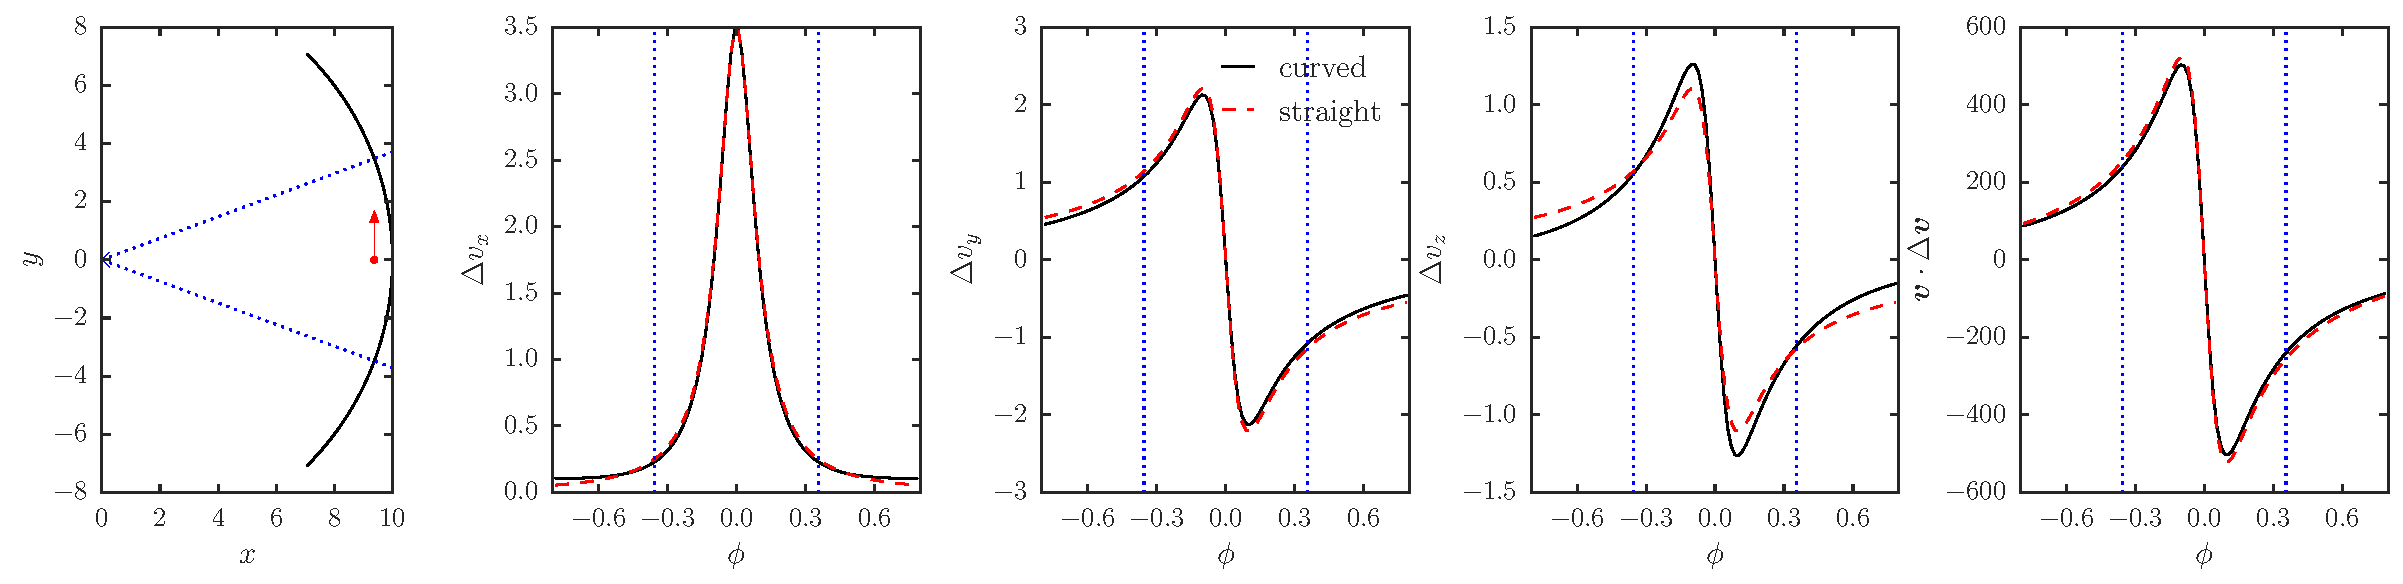
\includegraphics[width=\textwidth]{curved_straight_comparison}$$
\caption{
A comparison of the velocity kicks calculated assuming a straight stream track and using the true stream geometry. The stream track is a circular orbit of radius $10\kpc$ and circular velocity $220\kms$ and is shown in black in the left panel. The sub-halo is a Plummer sphere of mass $10^8M_\odot$ and scale radius $r_s=0.625\pc$ moving at $\bs{w}=(0,132,176)\kms$ with an impact parameter $b=r_s$. The red arrow shows the projection of the velocity vector into the plane. The second, third and fourth plots show the velocity kicks as a function of the azimuthal angle from the centre of the galaxy. The black lines show the kicks calculated using equation~\protect\eqref{curved} whilst the red dashed lines show the kicks computed assuming the stream is a straight line segment along the $y$-axis. The rightmost panel shows $\bs{v}\cdot\Delta\bs{v}$. The dotted blue lines show the angles at which the projection of the velocity vector of the sub-halo intersects the stream.
}
\label{curved_straight}
\end{figure*}

We also consider kicks due to truncated Navarro-Frenk-White profiles. The density profile for these halos is given by
\begin{equation}
\rho_{\rm NFW}(r) = \frac{M}{4\pi r_s^3}\Big(\frac{r}{r_s}\Big)^{-1}\Big(1+\frac{r}{r_s}\Big)^{-2}\mathrm{sech}\Big(\frac{r}{r_t}\Big).
\end{equation}
$r_t$ is the truncation radius. For non-zero $r_t$ the forces and potential must be computed numerically and clearly for $r_t\rightarrow\infty$ the form reduces to the well-known NFW profile. In Fig.~\eqref{plummer_nfw} we show the kicks computed for a Plummer sub-halo, NFW sub-halo and truncated NFW sub-halo. We also show $\bs{v}\cdot\Delta\bs{v}$ which is the quantity that controls the future structure of the stream. We have assumed the stream is a straight-line segment moving along the $y$ axis at velocity $v_y=2$. The Plummer sub-halo has $GM=2$, scale-radius $r_s=2$, impact parameter $b=\sqrt{3}$ and velocity $\bs{w}=(0.6,1.2,0)$. The NFW halo has the same mass parameter but the scale radius is chosen such that the mass contained within the Plummer scale radius is identical to the Plummer case. The truncated NFW profile has a truncation radius of $r_t=2$. The NFW profile is more spatially extended so the amplitude of the kicks are larger than the Plummer kicks at large distances from the impact. When the NFW profile is truncated the velocity kicks are very similar to the Plummer kicks.

\begin{figure*}
$$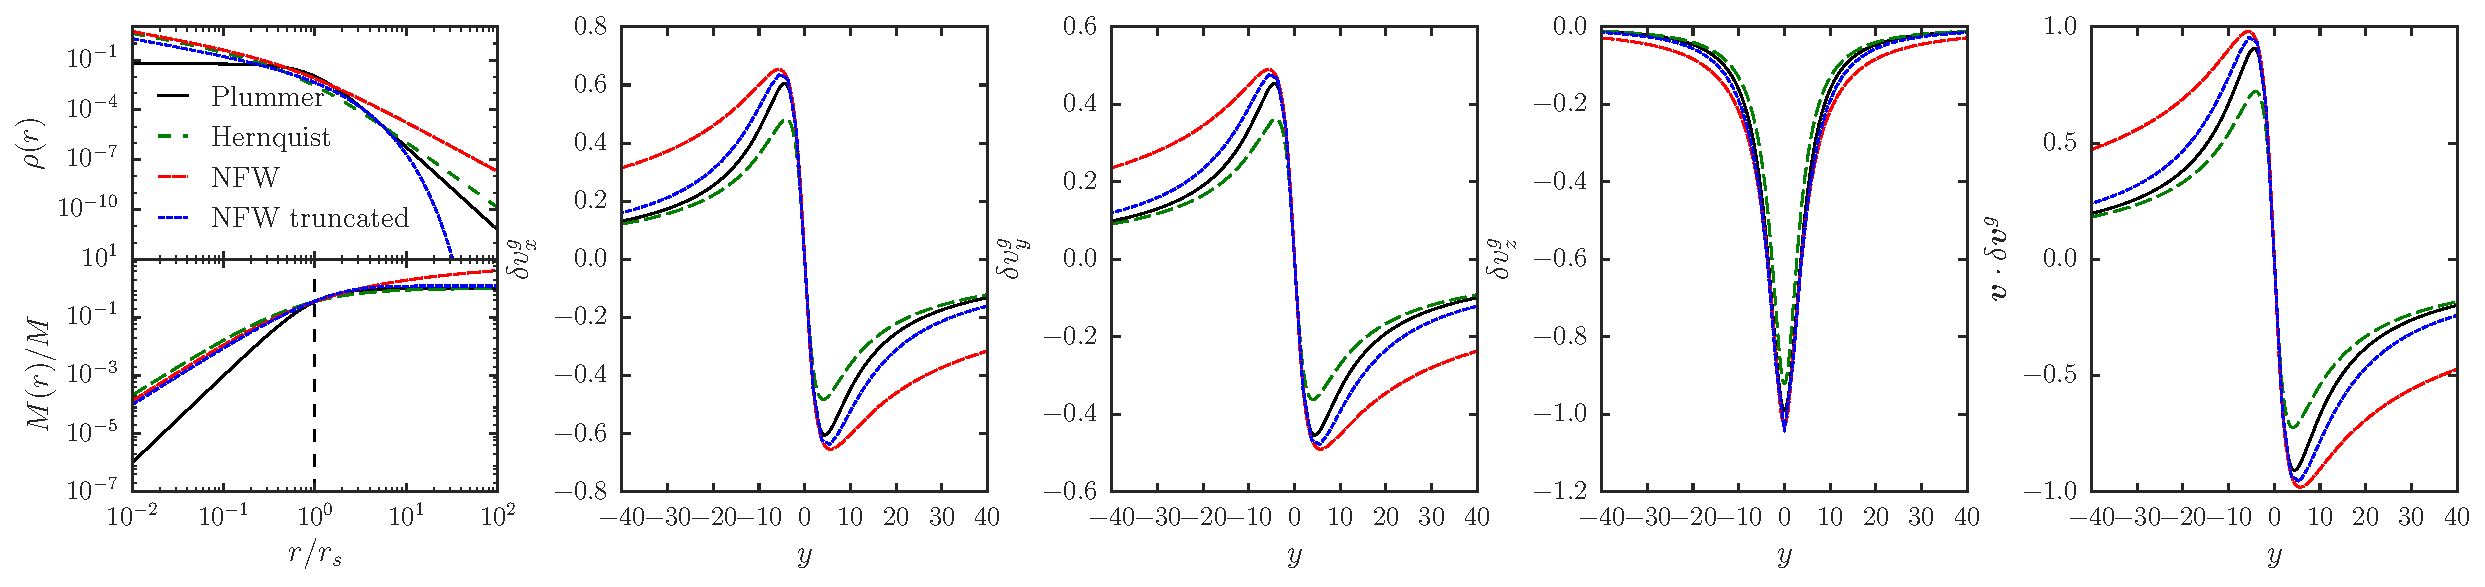
\includegraphics[width=\textwidth]{nfw_plummer_comparison}$$
\caption{
A comparison of the velocity kicks from a Plummer, a NFW and a truncated NFW sub-halo. The left panel shows the density and mass profiles of the three haloes. All three haloes have the same mass parameter but the NFW scale radius is chosen such that at the Plummer scale radius ($r_s$) the same mass is enclosed by both profiles. The truncated NFW halo has a scale radius equal to that of the Plummer sphere and a truncation radius of $2r_s$. The mass profiles for the three haloes are shown in the lower left panel. The second, third and fourth panels show the velocity kicks as a function of the distance along the stream. The rightmost panel shows $\bs{v}\cdot\Delta\bs{v}$. The stream is a particle train along the $y$-axis with velocity $2$. The sub-haloes have $GM=2$, $r_{s,\mathrm{Plummer}}=2,r_{s,\mathrm{NFW}}=1.21$
, impact parameter $b=\sqrt{3}$ and velocity $\bs{w}=(0.6,1.2,0)$. The velocity kicks have approximately the same amplitude and the key difference is the velocity kicks due to the NFW halo fall off more slowly with $|y|$ as the NFW halo is more spatially extended.
}
\label{plummer_nfw}
\end{figure*}

\subsection{Angle-frequency kicks}\label{Sec::Formalism_angfreq}
\cite{ErkalBelokurov} gave analytic results for the structure of a gap as a function of time for streams on circular orbits. Such an approach is fruitful for developing an understanding of the gap formation but when modelling realistic streams we require a formalism that is appropriate for eccentric orbits. Dynamical systems are often simplified through the use of angle-actions coordinates $(\bs{J},\btheta)$. These canonical coordinates possess the properties that the actions are integrals of motion whilst the angles increase linearly with time at a rate $\boldsymbol{\Omega}$, the frequencies. \cite{HelmiWhite1999} and \cite{Tremaine1999} both discussed the evolution of a stream as a small action clump in angle-actions, which was built on by the work of \cite{EyreBinney2011}. \cite{SandersBinney2013} presented the idea that the angle-frequency distribution could be used as a probe of the galactic potential. These ideas were extended by both \cite{Bovy2014} and \cite{Sanders2014} who developed generative models for streams in angle-frequency space. This framework is ideal for the introduction of velocity perturbations due to a sub-halo.

Each particle in a stream obeys the equation
\begin{equation}
\Delta\bs{\theta} = \btheta-\btheta_0 = (\boldsymbol{\Omega}-\boldsymbol{\Omega}_0)t_s +\Delta\bs{\theta}_\mathrm{init}= \Delta\bs{\Omega}_\mathrm{init}t_s,
\end{equation}
where the subscript $0$ denotes the coordinates of the progenitor, $\Delta$ denotes separation between the progenitor and a stream particle and $\mathrm{init}$ denotes the separation between progenitor and particle at release and $t_s$ is the time since the particle was stripped.

A long thin stream is characterised by a vector $\bs{n}$ along which the particles lie in both angle and frequency space. This vector is the principal eigenvector of the Hessian matrix $D_{ij}=\partial^2 H/\partial J_i\partial J_j$. Note that if the frequencies are functions solely of the Hamiltonian (as in the Kepler case) $\bs{n}$ is aligned with the stream particle frequency vectors and the stream is well approximately by an orbit. We will return to this point later. \cite{Bovy2014} and \cite{Sanders2014} introduced a model for each tail of the stream (leading or trailing) in angle-frequency space that was an elongated Gaussian in the frequency offset from the progenitor and a isotropic Gaussian in initial angle offset from the progenitor. By estimating some stripping rate $p(t)$ the angle-frequency distribution could be calculated at all times. Through the introduction of a linear transformation from position-velocity space to angle-frequency space in the neighbourhood of the stream, \cite{Bovy2014} demonstrated that the stream model could be rapidly sampled at any time.

The angle-frequency model of a stream can be simply extended to include the effects of a gap. Under the impulse approximation of the previous section we can calculate the change to the angles and frequencies for small velocity kicks as
\begin{equation}
\begin{split}
\delta \boldsymbol{\Omega}^g &= \frac{\upartial \boldsymbol{\Omega}}{\upartial \bs{v}}\Big|_{\bs{x}}\cdot \delta\bs{v},\\
\delta \bs{\theta}^g &= \frac{\upartial \bs{\theta}}{\upartial \bs{v}}\Big|_{\bs{x}}\cdot \delta\bs{v}.
\end{split}
\end{equation}
The stream stretches along the direction $\bs{n}$ and in each tail the frequency distribution is very narrow such that, at a fixed time, the location of the particles in the stream are well approximated by a single angle coordinate $\theta_{||}=\btheta\cdot\bs{n}$. We assume that the kicks are functions of this single variable. If the kick occurred a time $t_g$ ago the angles and frequencies of a stream particle are given by
\begin{equation}
\begin{split}
\Delta\bs{\theta} &= \Delta\bs{\theta}_{\rm init}+\Delta\boldsymbol{\Omega}_{\rm init}(t_s-t_g)+\delta\bs{\theta}^g+(\Delta\boldsymbol{\Omega}_{\rm init}+\delta\boldsymbol{\Omega}^g)t_g \\&= \Delta\bs{\theta}_{\rm init}+\Delta\boldsymbol{\Omega}_{\rm init}t_s+\delta\bs{\theta}^g+\delta\boldsymbol{\Omega}^g t_g.
\end{split}
\end{equation}
The particle moves with its initial frequency separation until the kick at which point the particle continues to move at the initial frequency separation plus the frequency kicks.

The matrices $\frac{\upartial \bs{\theta}}{\upartial \bs{v}}\Big|_{\bs{x}}$ and $\frac{\upartial \bs{\Omega}}{\upartial \bs{v}}\Big|_{\bs{x}}$ must be calculated numerically. However, we will demonstrate that there are several approximate analytic relations that hold well for the inspected simulation.

\section{Simulation}\label{sect::simulation}
We use two simulations to investigate the formation of stream gaps in actions, angles and frequencies. Here we describe the set-up of the simulations. The stream progenitor is a King profile globular cluster with $W_0=5$, a mass of $10^5 M_\odot$ and a core radius of $r_c=13\pc$. The cluster was modelled with $10^6$ particles and a smoothing length of $1\pc$.
The galactic potential was modelled as a logarithmic halo of the form
\begin{equation}
\Phi_\mathrm{L}(R,z) = \frac{V_c^2}{2}\log\Big(R^2+\frac{z^2}{q^2}\Big),
\end{equation}
with $V_c = 220\kms$ and $q = 0.9$. The cluster was placed on two different orbits -- one with zero $J_z$ and one with non-zero $J_z$. Both orbits are eccentric with pericentre of $15\kpc$ and apocentre of $30\kpc$, and the clusters are released around apocentre at $(30,0,0)\kpc$. The zero $J_z$ simulation uses an initial velocity of $(0,149.55,0)\kms$ and the non-zero $J_z$ uses an initial velocity of $(0, 105.75, 105.75)\kms$. Both simulations were run for $10\Gyr$ and the stream was then impacted with a Plummer sub-halo of mass $10^8M_\odot$ and scale radius $r_s=625\pc$. The impact point in both cases was near pericentre with a impact parameter of $b=0$ and the velocity is perpendicular to the stream plane at this point with magnitude of $200\kms$. The sub-halo was inserted into the simulations $100\Myr$ before impact and removed $100\Myr$ after impact. Both simulations were then evolved for a further $5\Gyr$. The simulations were run using \textsc{Gadget}. In Figure~\ref{GapDiagram} we show the full non-zero $J_z$ stream in the $(x,y)$ plane and a zoom-in of the gap centre at $880\Myr$ after impact.

\begin{figure}
$$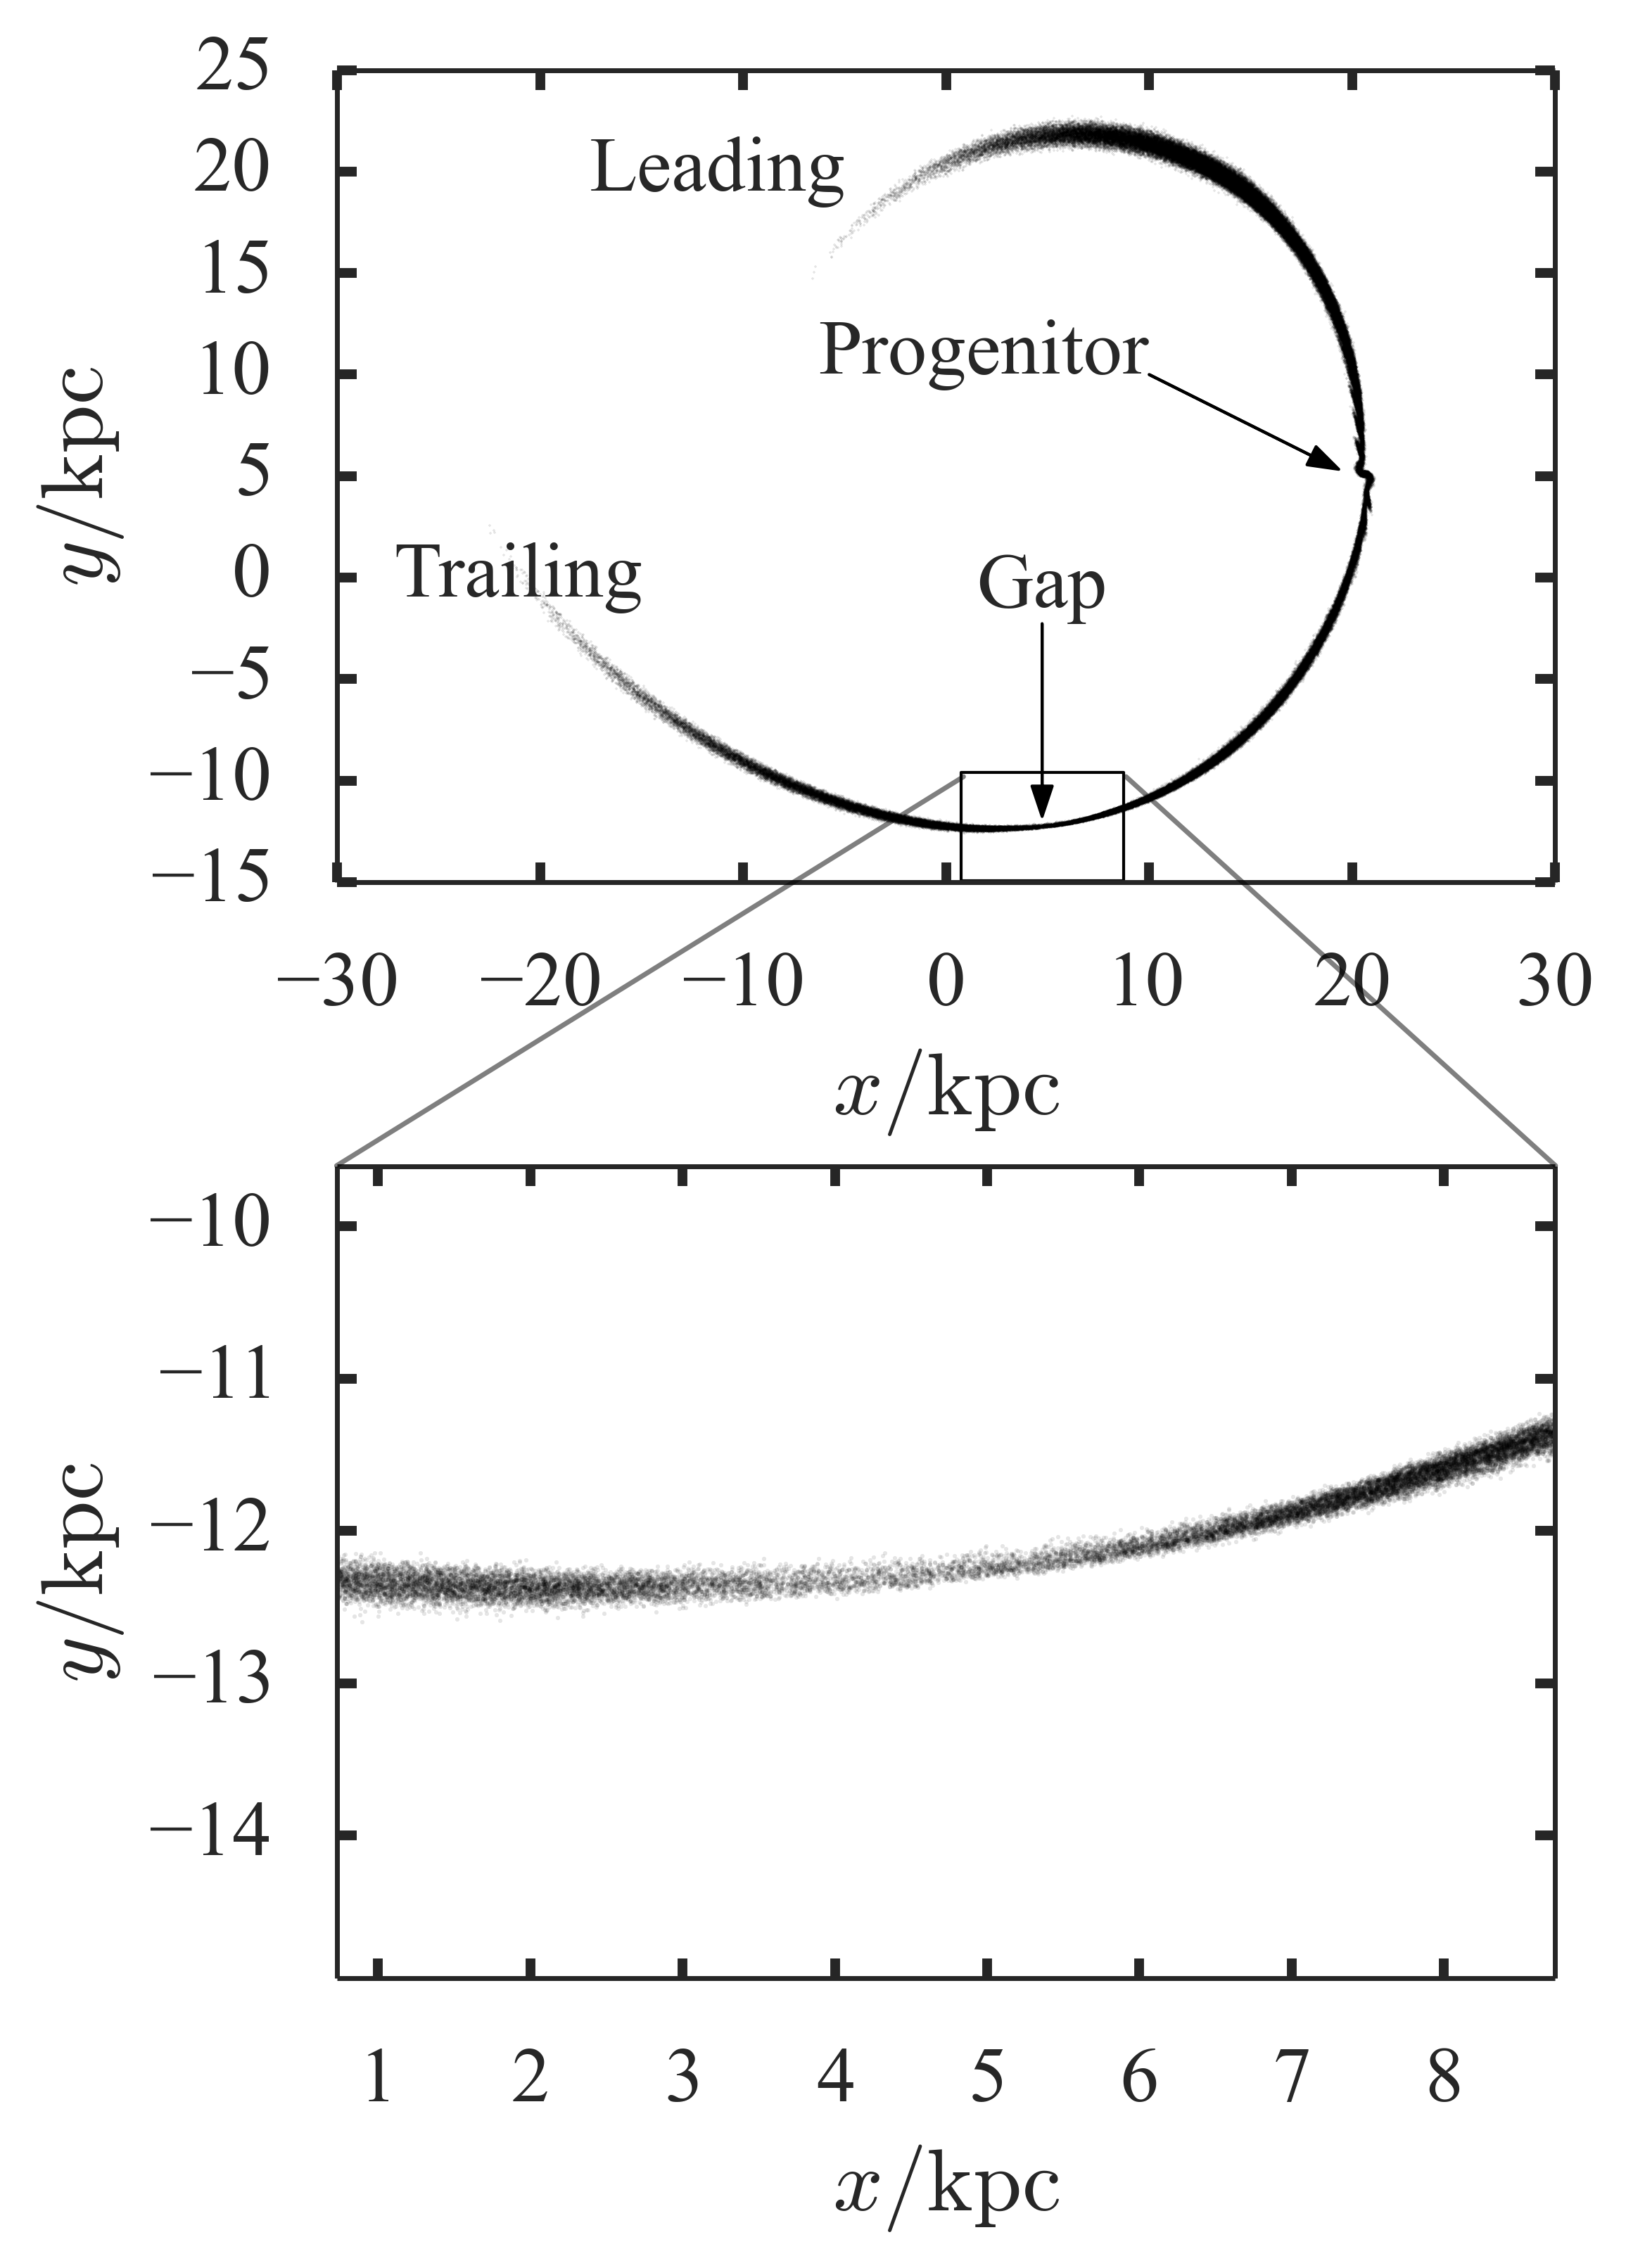
\includegraphics[width=\columnwidth]{tilted_gap_morphology}$$
\caption{
Real-space distribution of stream and gap zoom-in.
}
\label{GapDiagram}
\end{figure}

\subsection{Action, angle \& frequency structure}
Here we investigate the angle, action and frequency structure of the stream. We take the snapshot of the zero-$J_z$ stream at $870\Myr$ after impact and the non-zero-$J_z$ stream at $880\Myr$ after impact and compute the angles, frequencies and actions for all particles in the trailing stream tail (defined by a spatial cut) XXX NOT TRUE FOR ZERO JZ STREAM -- I THINK IT IS THE LEADING TAIL AND I HAVE NOT COMPUTED THE QUANTITIES FOR ALL PARTICLES IN THE TAIL XXX. We also perform the same calculation for the stream evolved without a sub-halo flyby. In Fig.~\ref{diff_map} we show histograms of the difference in the density in angle, frequency and action space for the zero-$J_z$ simulation. We suppress the $z$ quantities as they are not informative due to the special nature of the progenitor orbit. In Fig.~\ref{tilted_diff_map} we show the equivalent plots for the non-zero-$J_z$ simulation. We plot all quantities with respect to the coordinates of the gap centre which is defined by eye. In the angle and frequency distributions there is a clear under-density along the stream direction. In action space we also observe an under-density at the centre of the distributions but the exact geometry of the under and over-densities clearly depends on the nature of the stream track and sub-halo properties. We will discuss this further later.

\begin{figure}
$$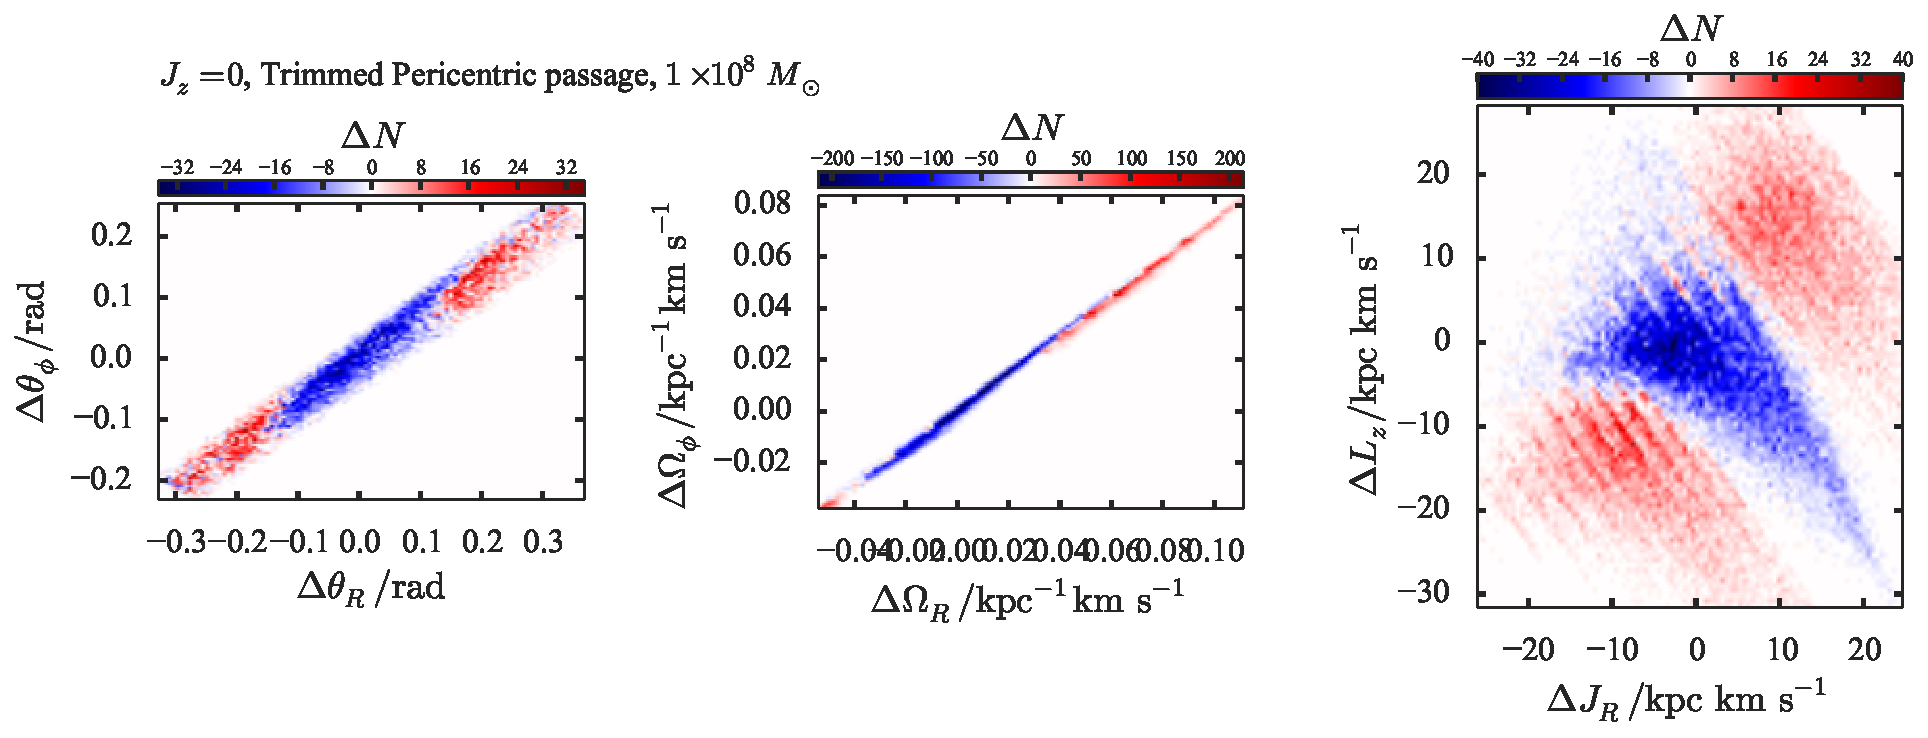
\includegraphics[width=\columnwidth]{diff_map}$$
\caption{
Difference histograms between the unperturbed and perturbed streams for the $J_z=0$ progenitor with respect to the gap centre. The left panel shows the distribution in angles, middle panel frequencies and right panel actions.
}
\label{diff_map}
\end{figure}

\begin{figure}
$$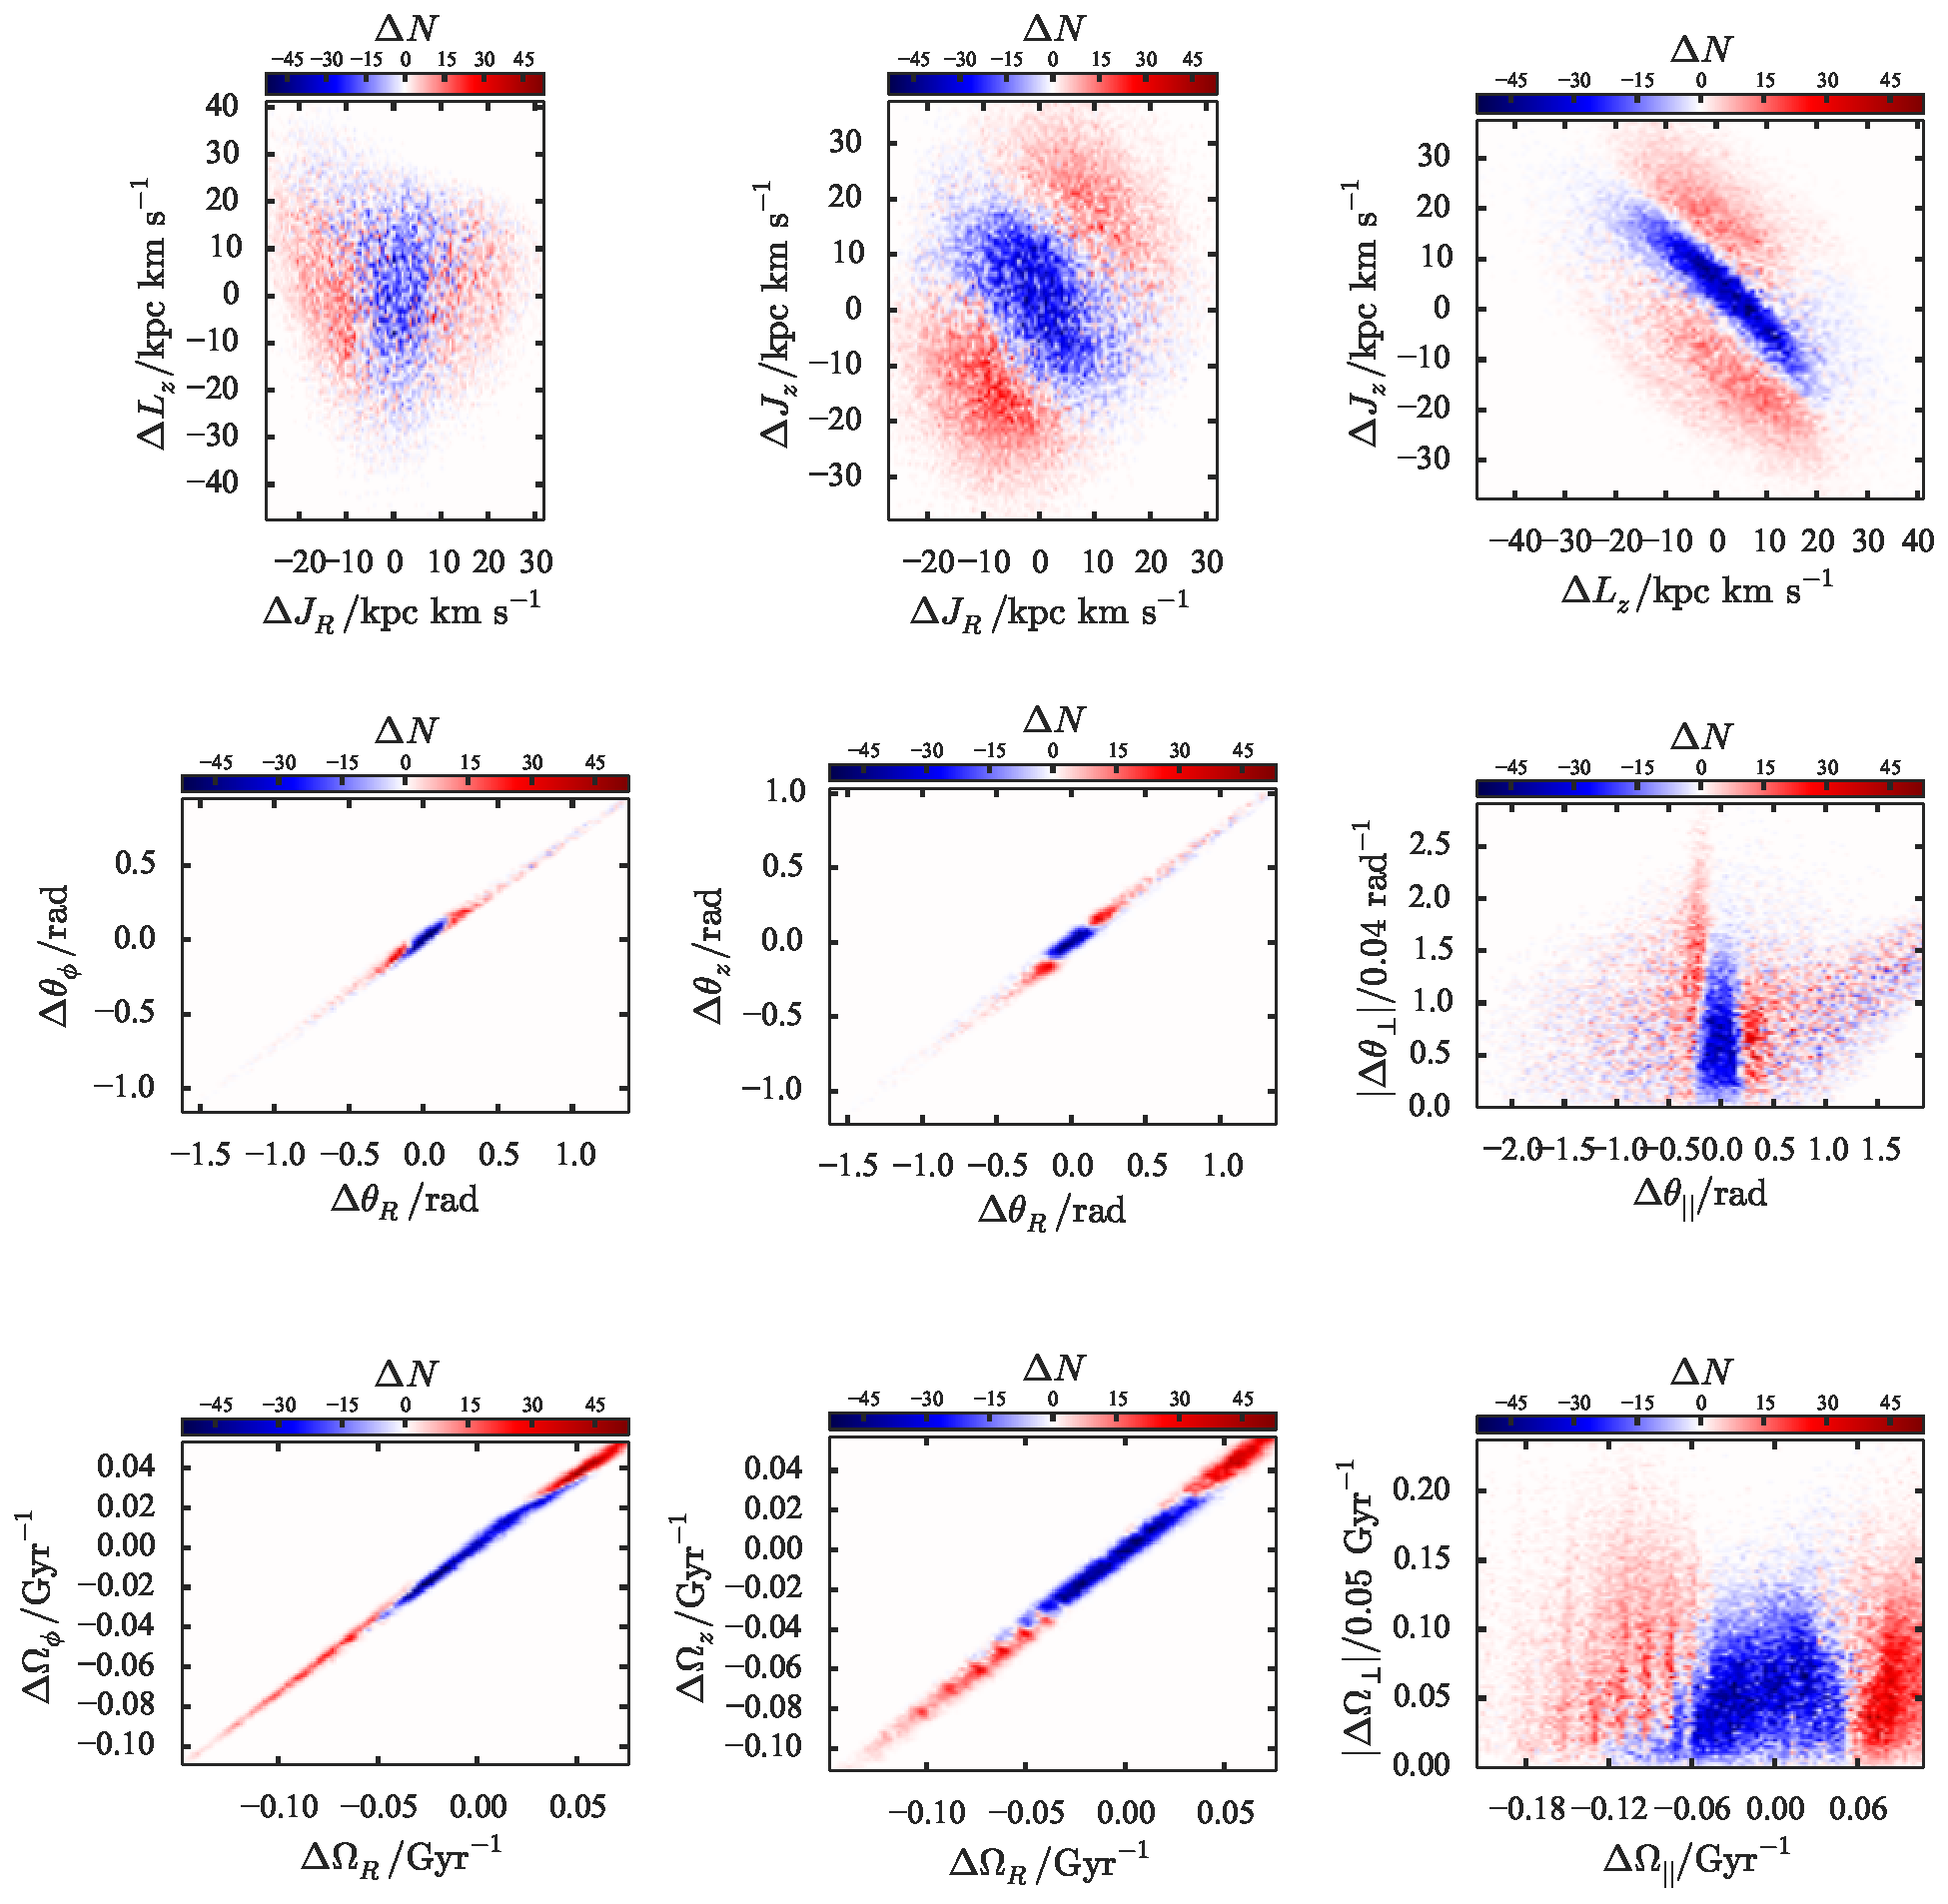
\includegraphics[width=\columnwidth]{tilted_diff_map}$$
\caption{
Difference histograms between the unperturbed and perturbed streams for the $J_z\neq0$ progenitor. The left panel shows the distribution in angles, middle panel frequencies and right panel actions.
}
\label{tilted_diff_map}
\end{figure}

\begin{figure}
$$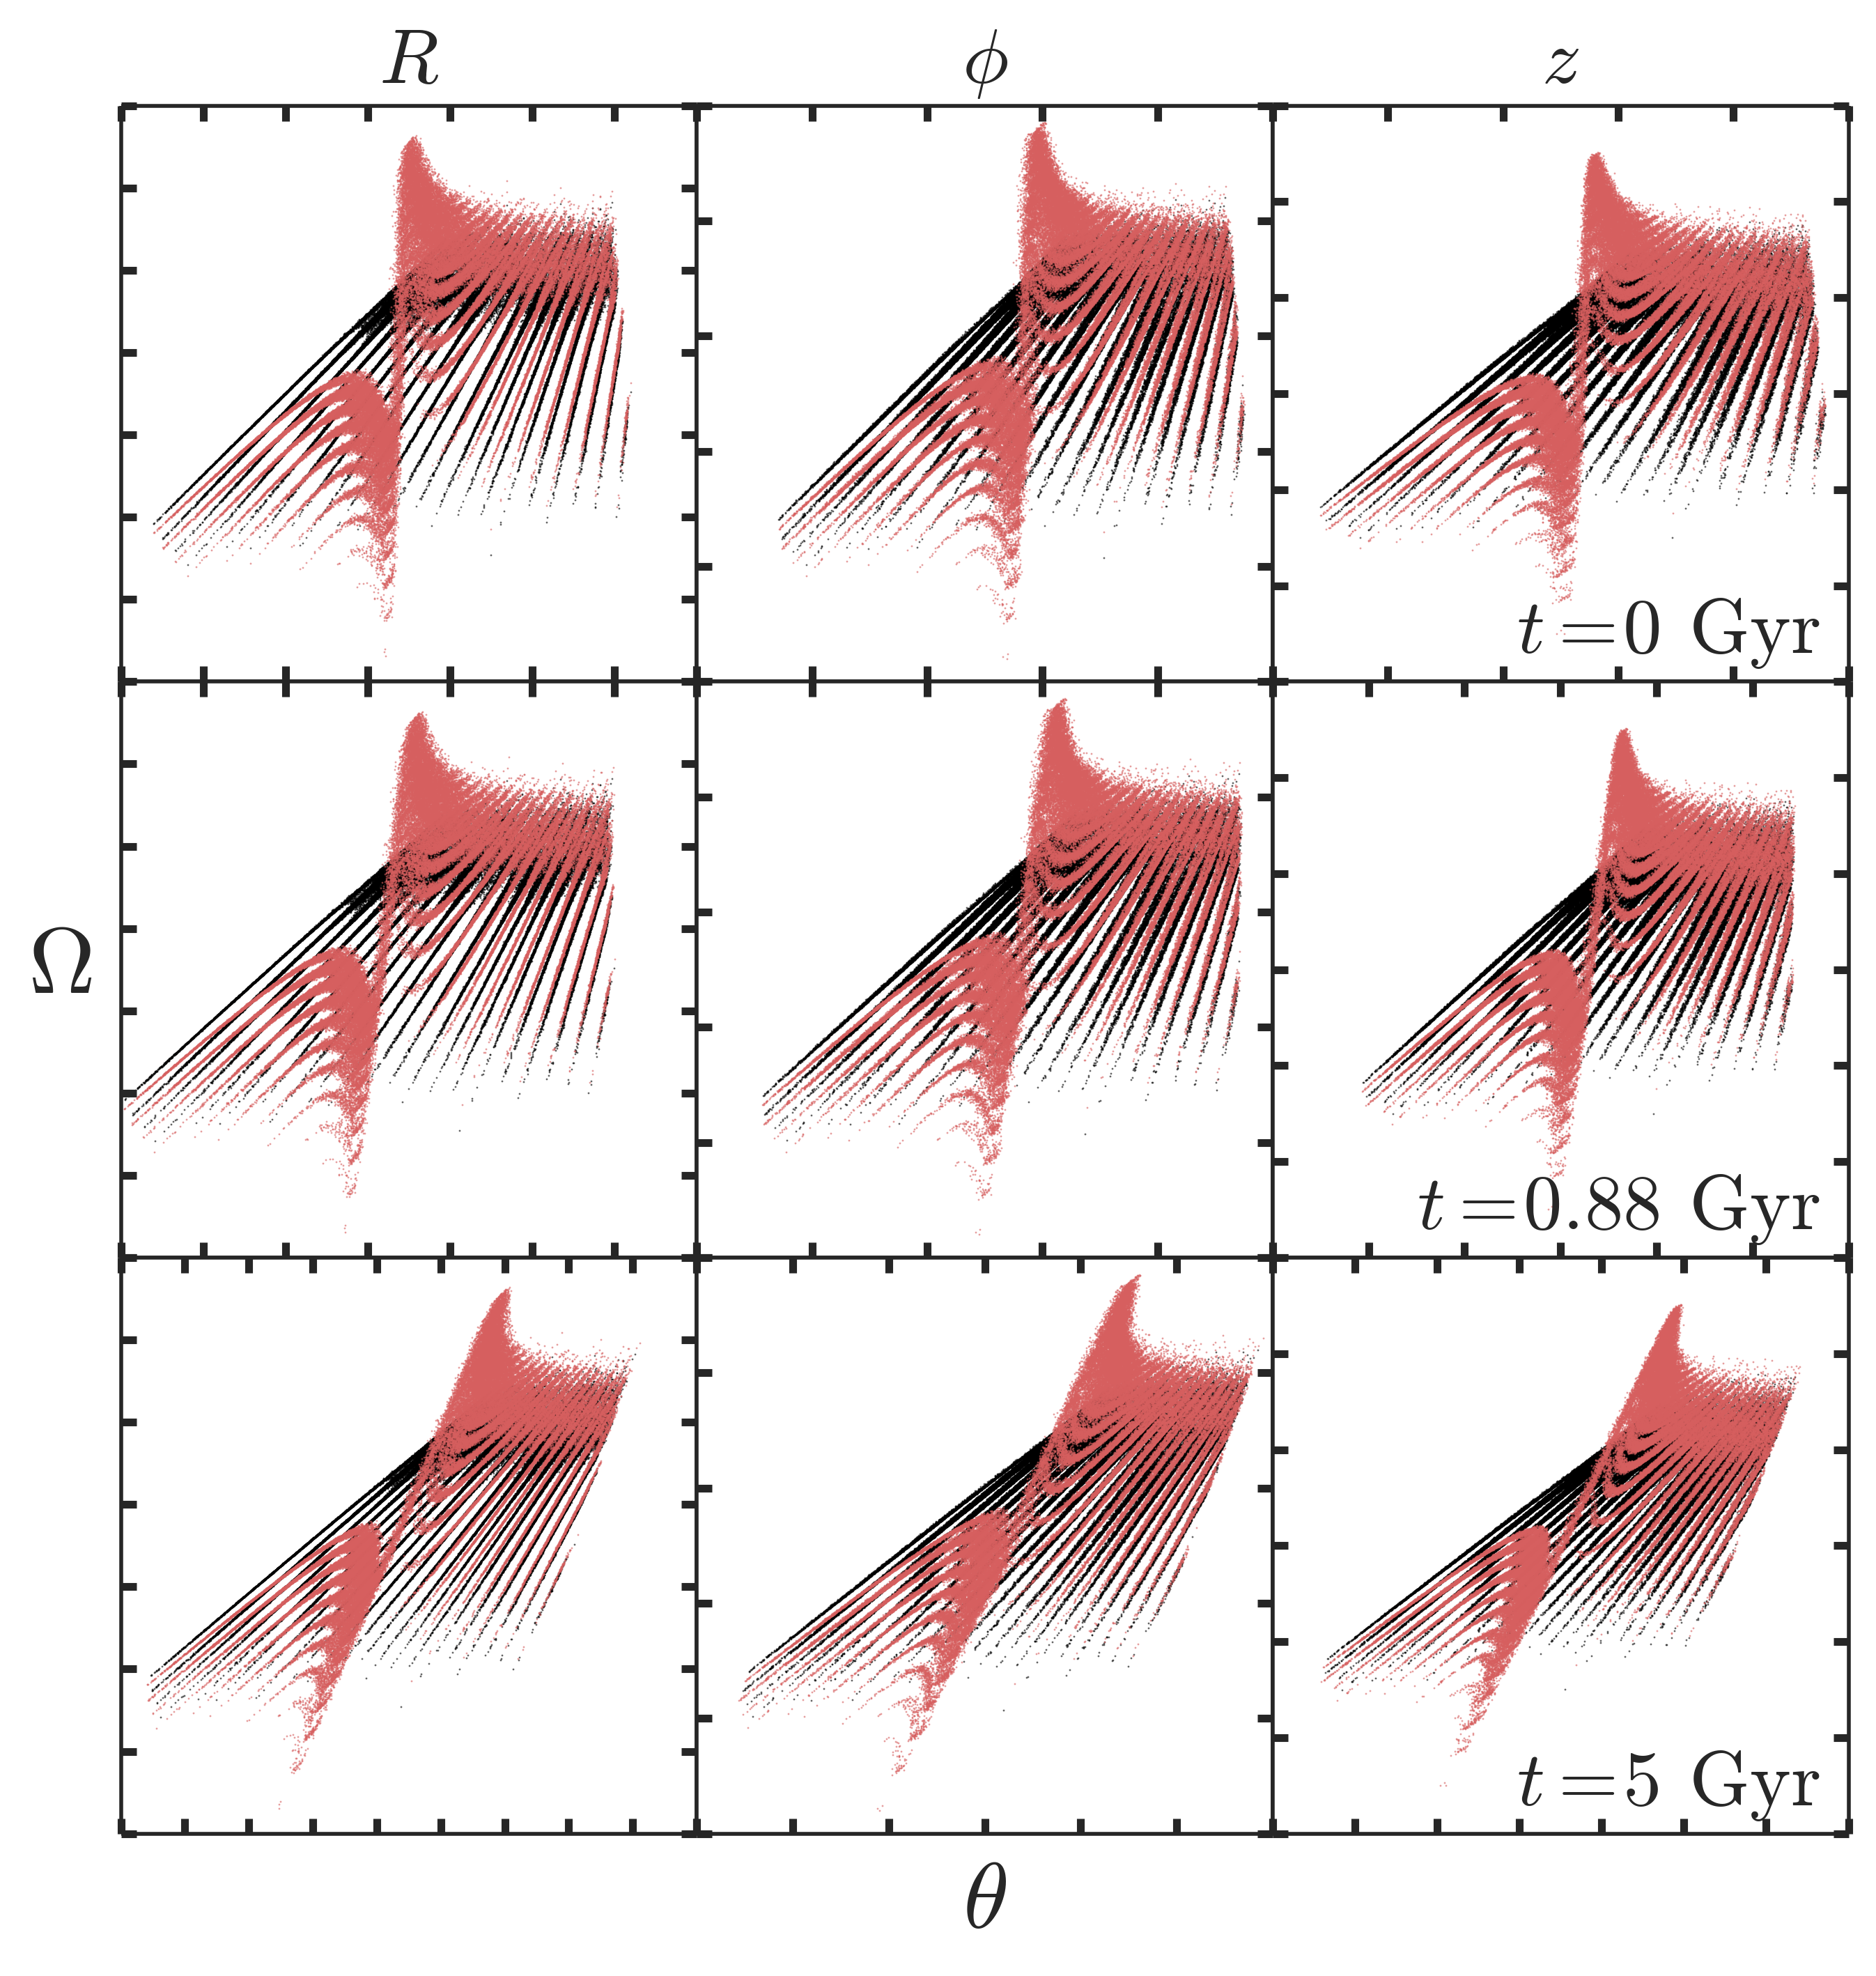
\includegraphics[width=\columnwidth]{ang_freq_dists}$$
\caption{
Frequency-angle distributions for unperturbed and perturbed trailing tail at three different times.
}
\label{angfreq_dist}
\end{figure}

\subsection{Kicks}
In Section~\ref{Sec::Formalism_angfreq} we described how the angle and frequency kicks due to a sub-halo can be computed under a linear approximation from the velocity kicks. Here we use the expressions and compare the resulting kicks with those measured from the simulation.

We begin by taking the snapshot of the unperturbed stream at the impact time and form a stream track by fitting a spline to the stream particles. We then compute the vector $\bs{n}$ from this track and at each point along the stream track compute $\theta_{||}=\btheta\cdot\bs{n}$ as well as $\delta\bs{\Omega}^g(\theta_{||})$ and $\delta\bs{\theta}^g(\theta_{||})$ by finite differencing in velocity at fixed position. We show the resultant kicks for the zero-$J_z$ stream in Fig.~\ref{kicks_zero} and for the non-zero-$J_z$ stream in Fig.~\ref{kicks_nzero}. We also show the angle and frequency kicks computed from the simulation. In the case of the frequency kicks we simply difference the perturbed and unperturbed simulation. In the case of the angles we must calculate the angles and frequencies of the perturbed simulation and rewind to the impact point before differencing with the unperturbed snapshot. Note the match is satisfactory and for both examples the angle kick dominates on time-scales $\sim100\Myr$ whilst the frequency kicks dominate beyond this.

\begin{figure}
$$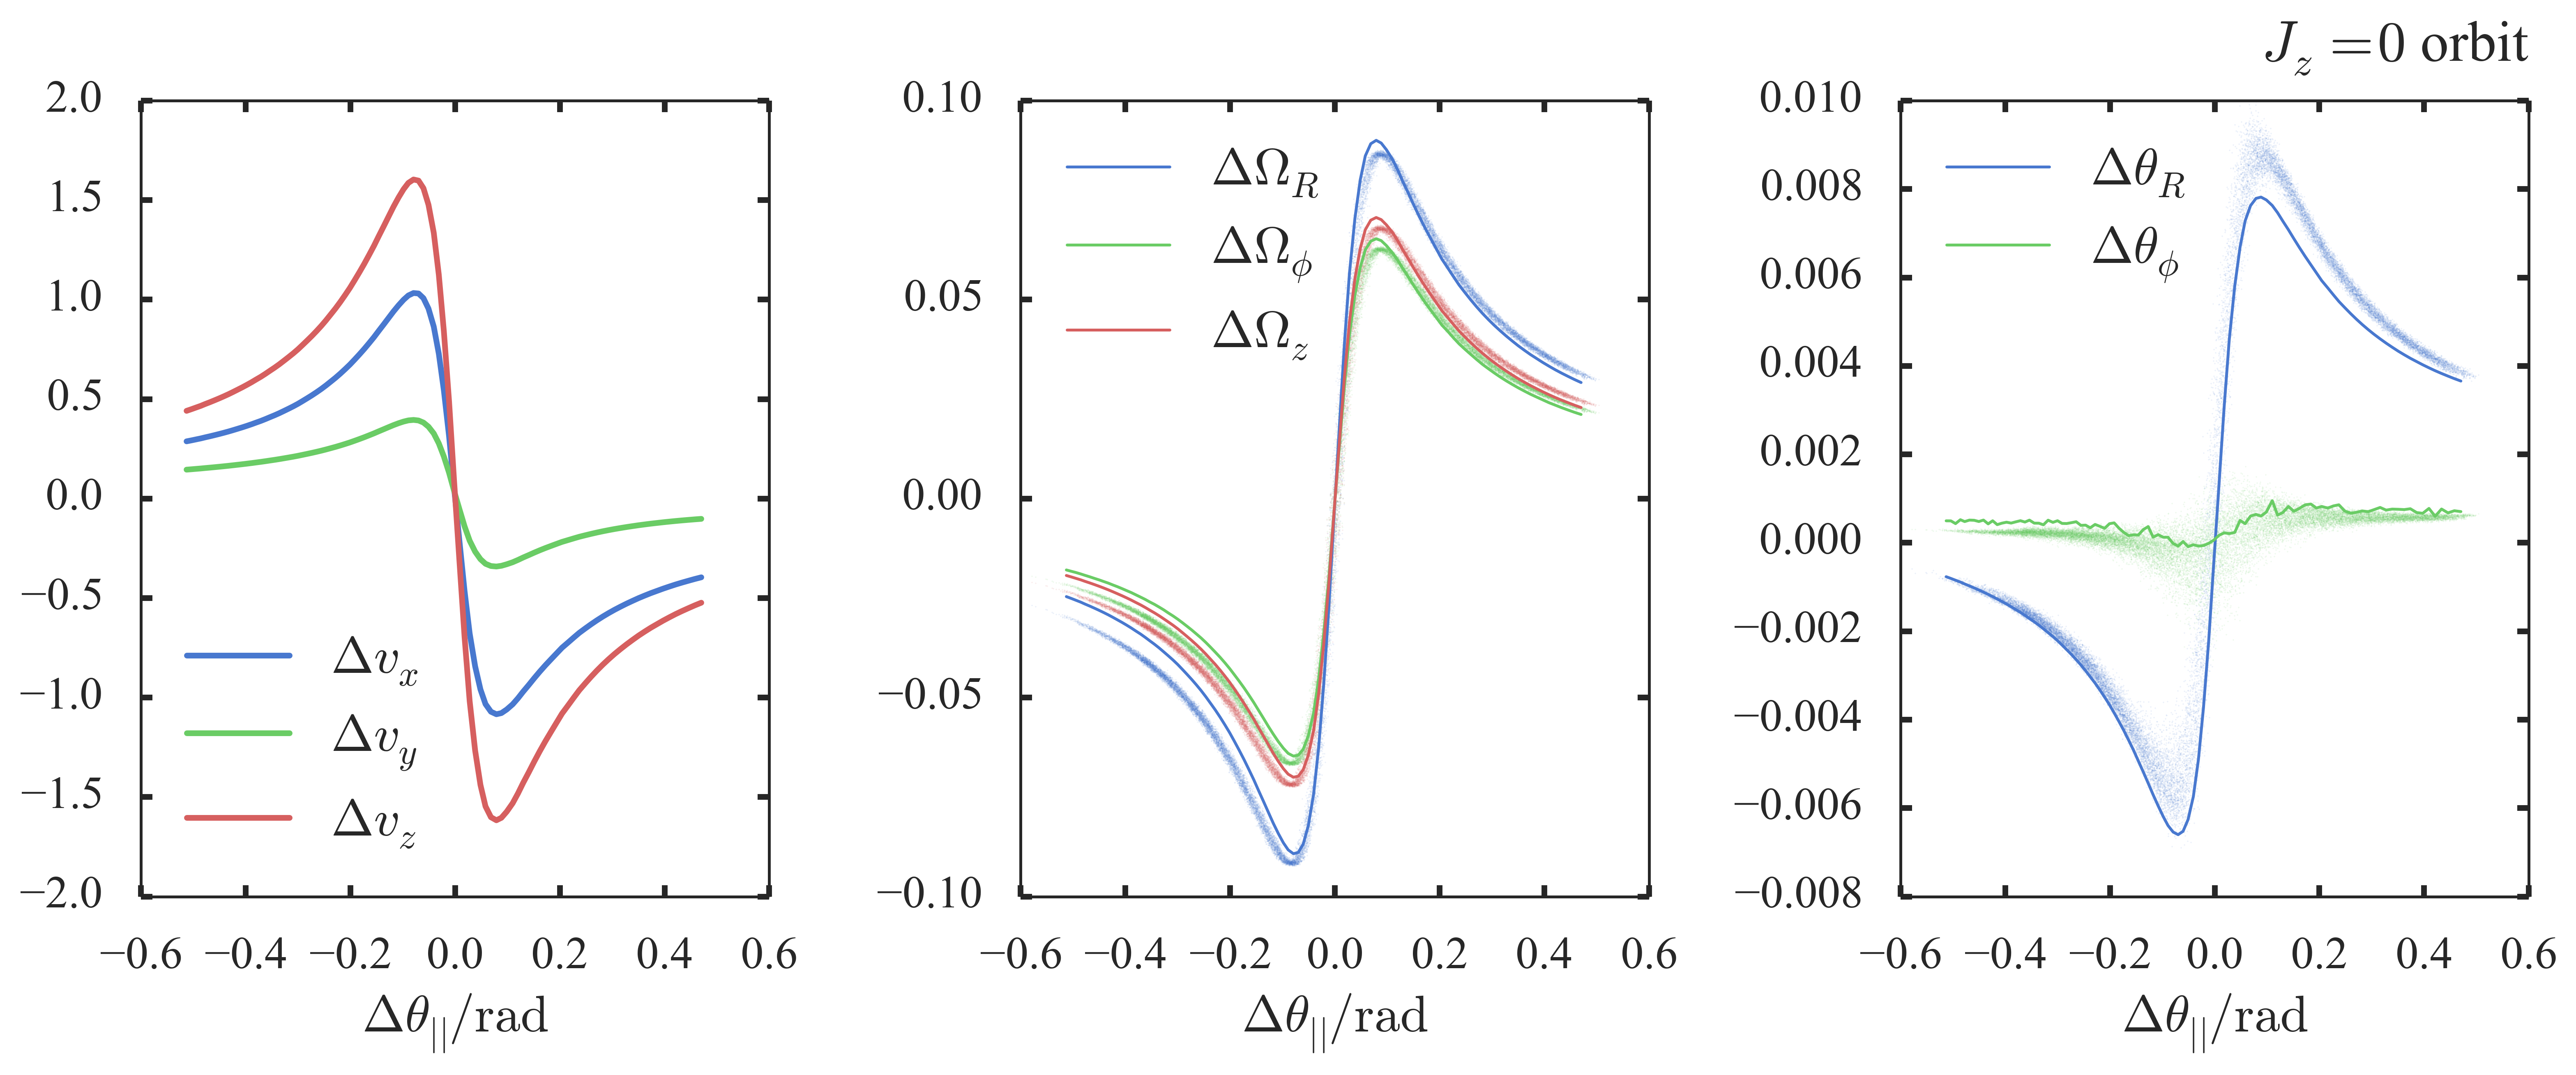
\includegraphics[width=\columnwidth]{angfreq_kicks.png}$$
\caption{
Angle and frequency kicks for the $J_z=0$ progenitor stream. The points show the kicks found from the simulations whilst the lines show those calculated under the impulse approximation.
}
\label{kicks_zero}
\end{figure}

\begin{figure}
$$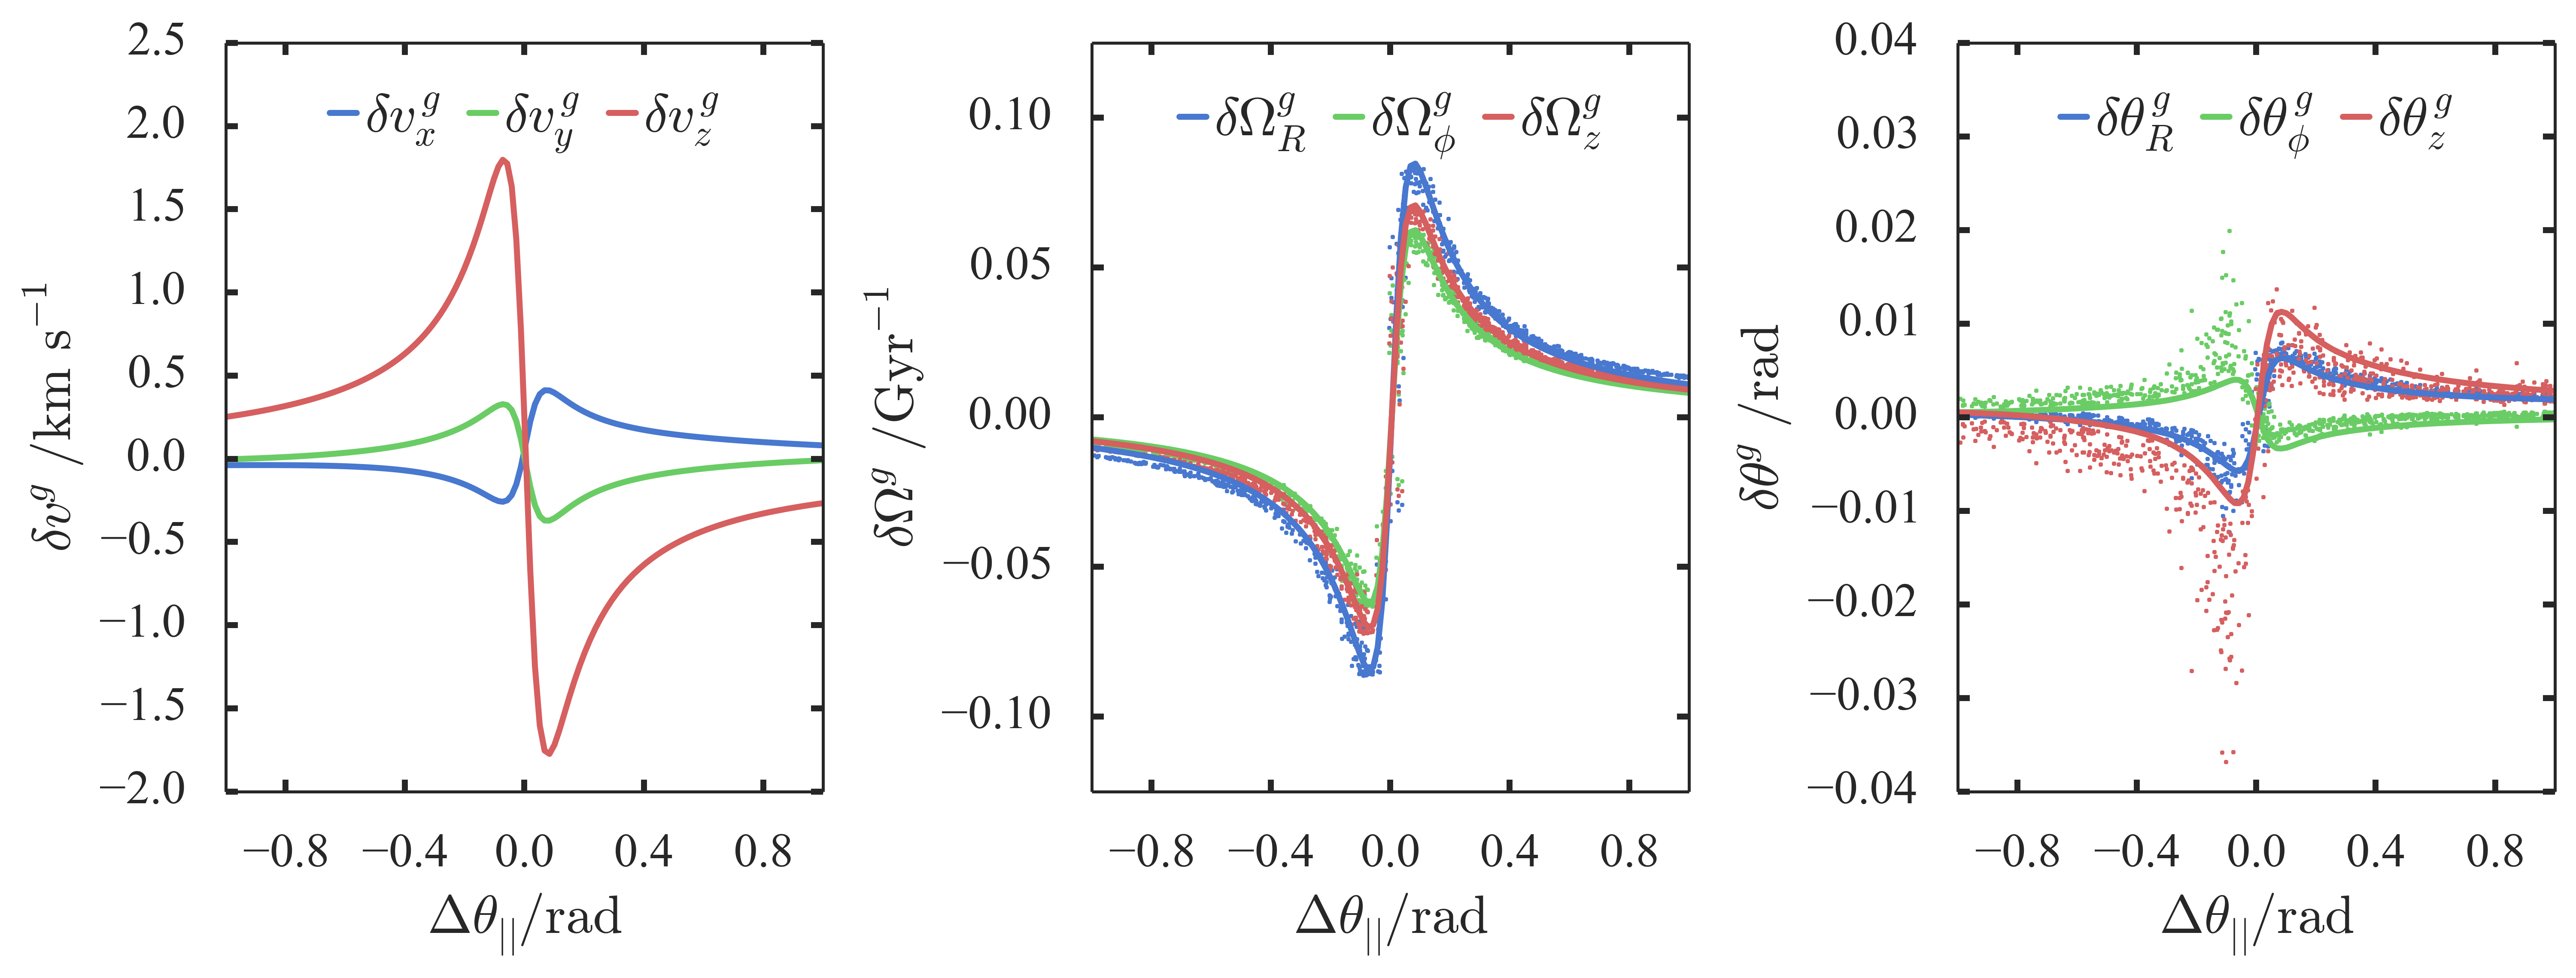
\includegraphics[width=\columnwidth]{tilted_angfreq_kicks.png}$$
\caption{
Angle and frequency kicks for the $J_z\neq0$ progenitor stream. The points show the kicks found from the simulations whilst the lines show those calculated under the impulse approximation.
}
\label{kicks_nzero}
\end{figure}

\subsection{Model-simulation comparison}
With the angle and frequency kicks satisfactorily calculated we proceed to take the unperturbed simulation, apply the kicks and compare with the perturbed simulation at later times.

In Fig.~\ref{model_zero} we show the angle and frequency distributions of the unperturbed simulation, the perturbed simulation and our model constructed by perturbing the angles and frequencies of the unperturbed simulation for the zero-$J_z$ stream after $870\Myr$. Similarly in Fig.~\ref{model_nzero} we show the results for the non-zero-$J_z$ stream after $880\Myr$. In both cases the match is very good (apart from $\theta_z$ for the zero-$J_z$ stream which is awkward due to the special stream geometry) and there is a clear gap in both angle and frequency.

\begin{figure}
$$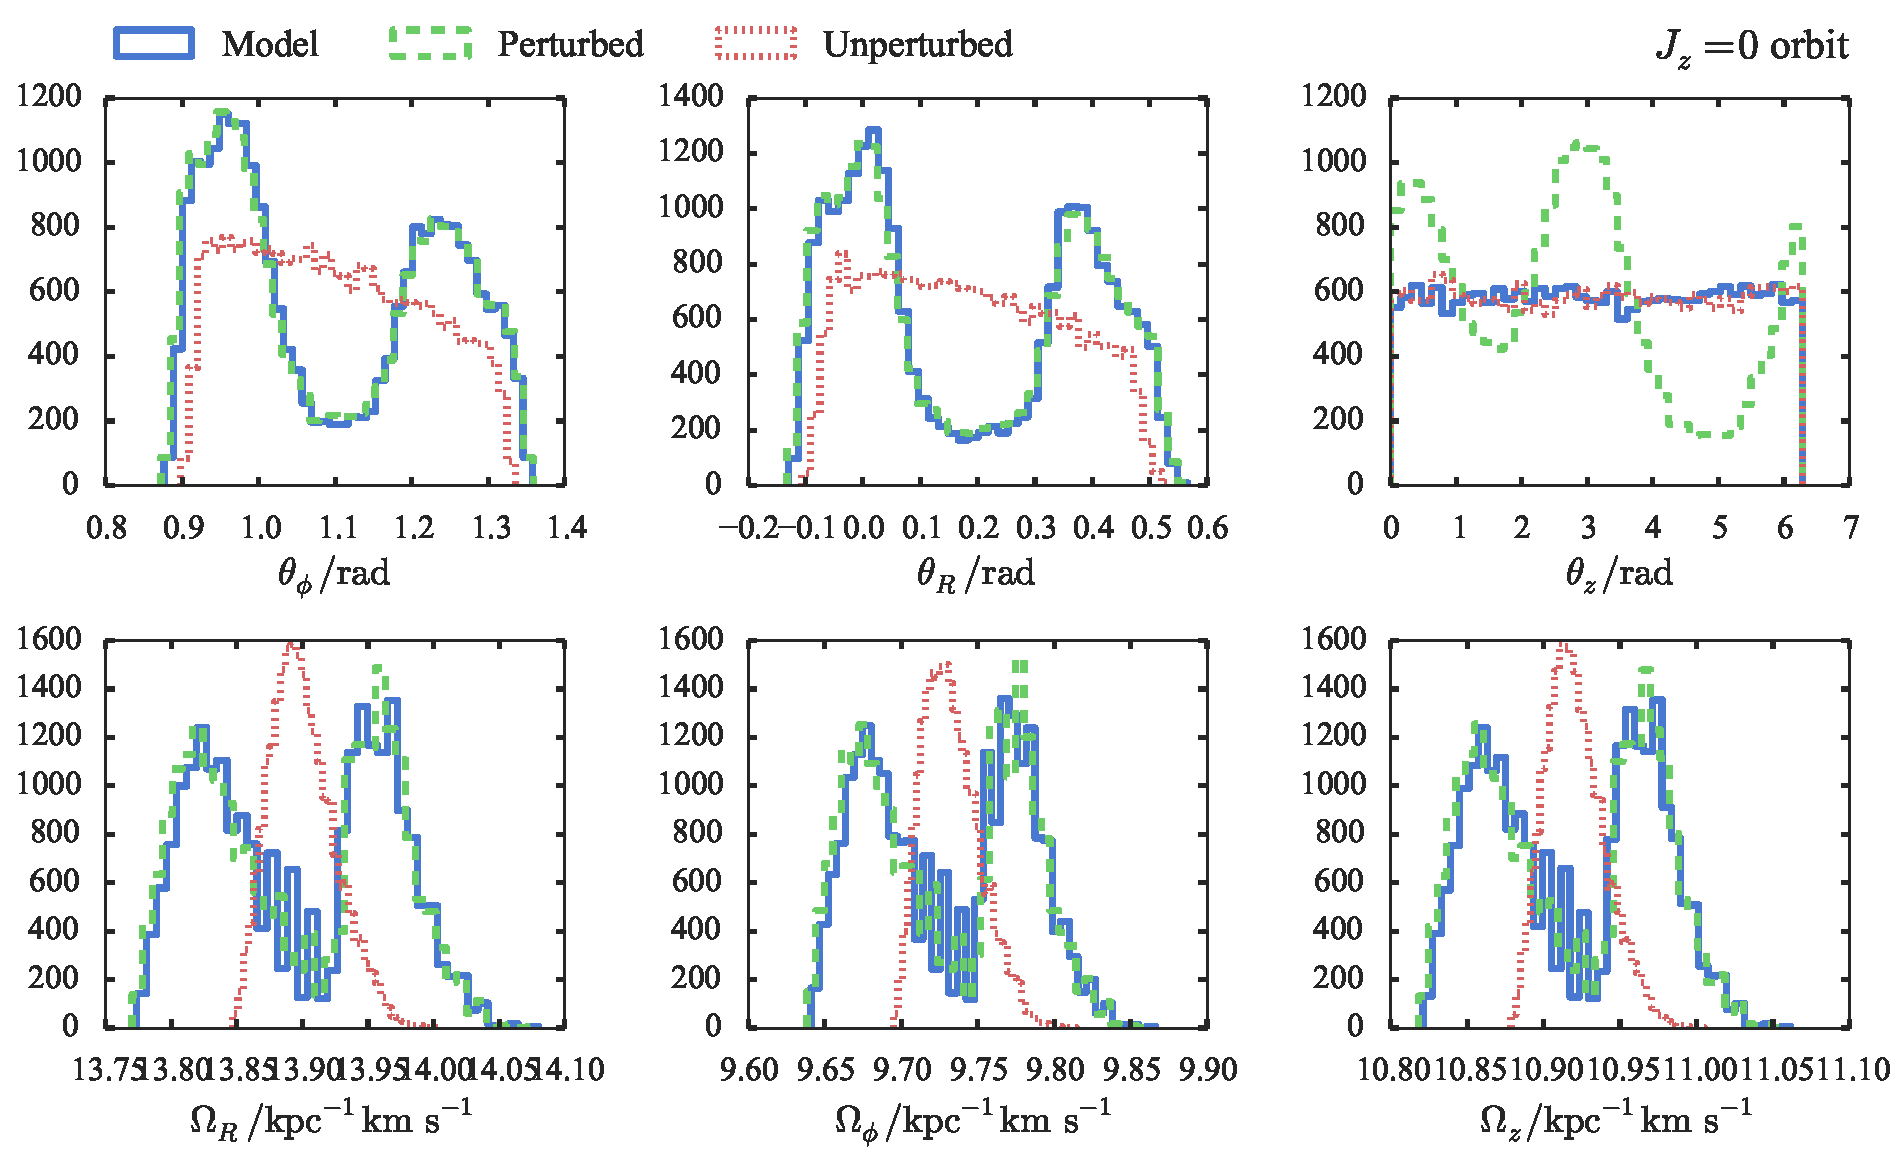
\includegraphics[width=\columnwidth]{model_perturbed}$$
\caption{
Unperturbed, perturbed and model stream for the $J_z=0$ progenitor. The red histograms show the unperturbed stream at the current time, the green show the perturbed stream and the blue show the unperturbed stream kicked in angle and frequency space and evolved to the current time.
}
\label{model_zero}
\end{figure}

\begin{figure}
$$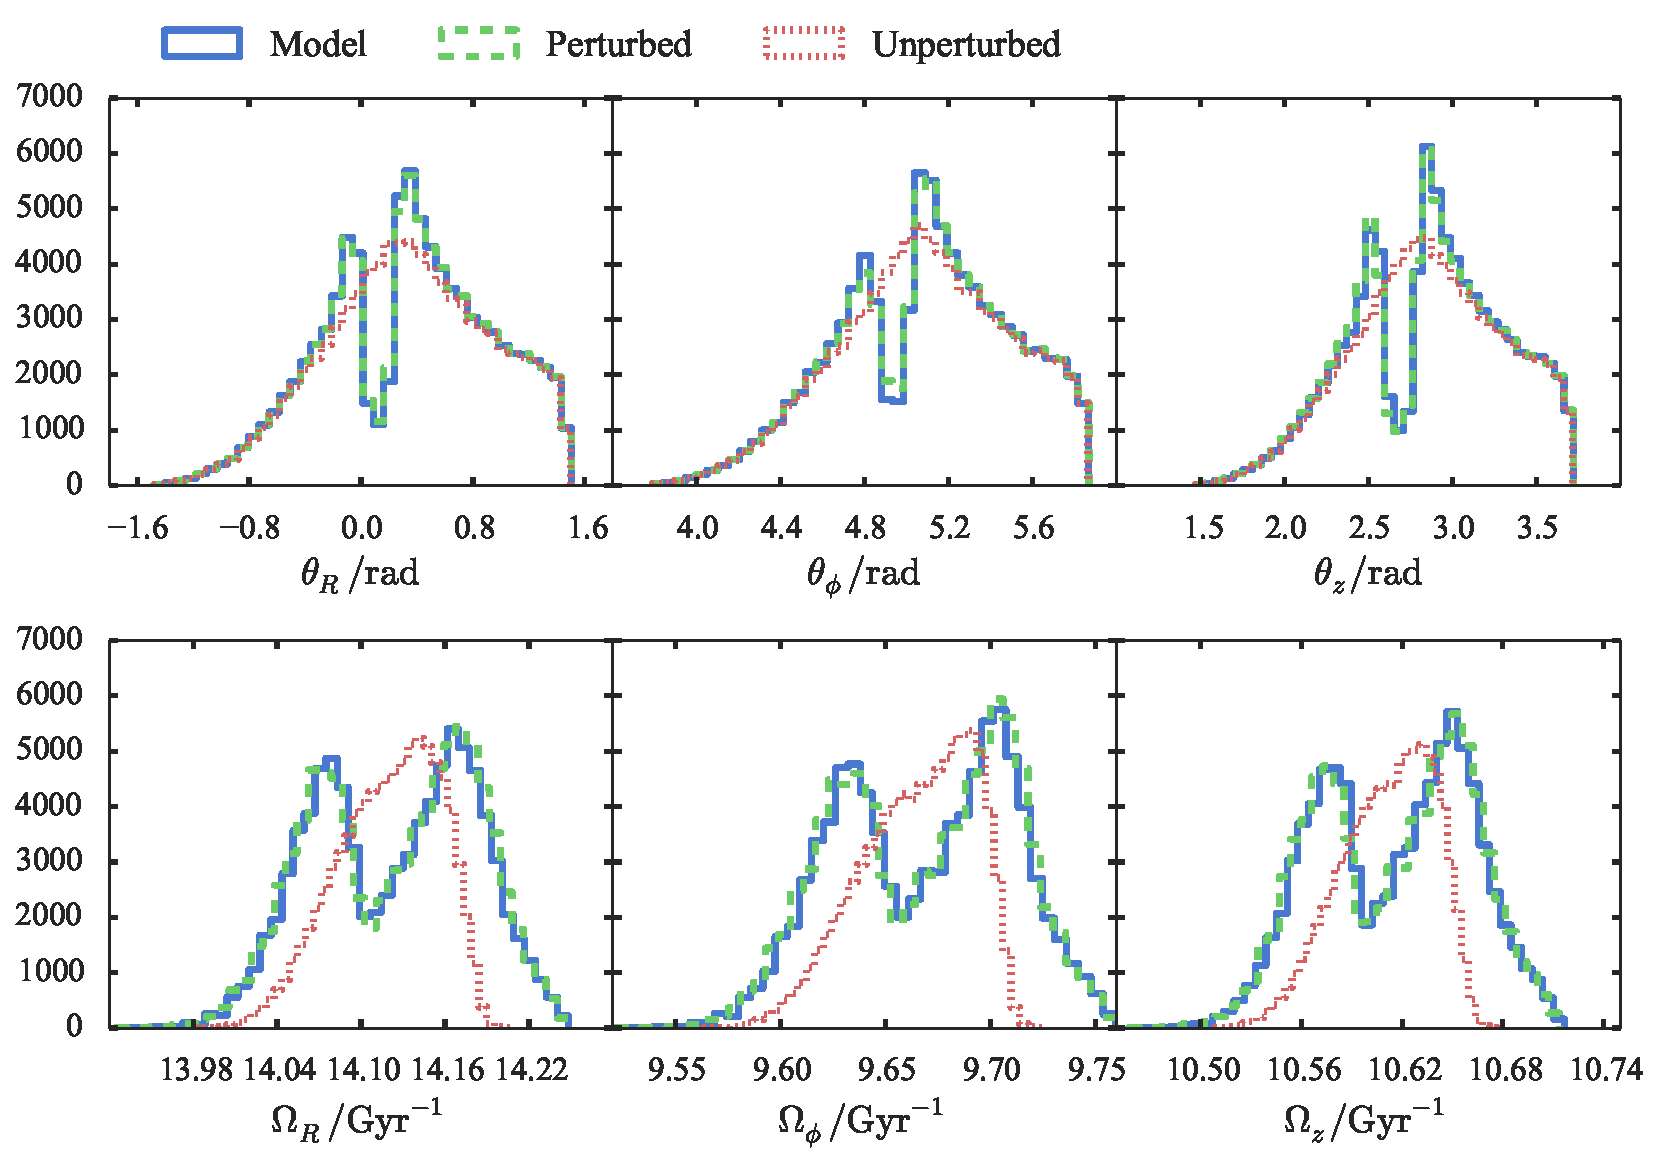
\includegraphics[width=\columnwidth]{tilted_model_perturbed}$$
\caption{
Unperturbed, perturbed and model stream for the $J_z\neq0$ progenitor. The red histograms show the unperturbed stream at the current time, the green show the perturbed stream and the blue show the unperturbed stream kicked in angle and frequency space and evolved to the current time.
}
\label{model_nzero}
\end{figure}

\begin{figure}
$$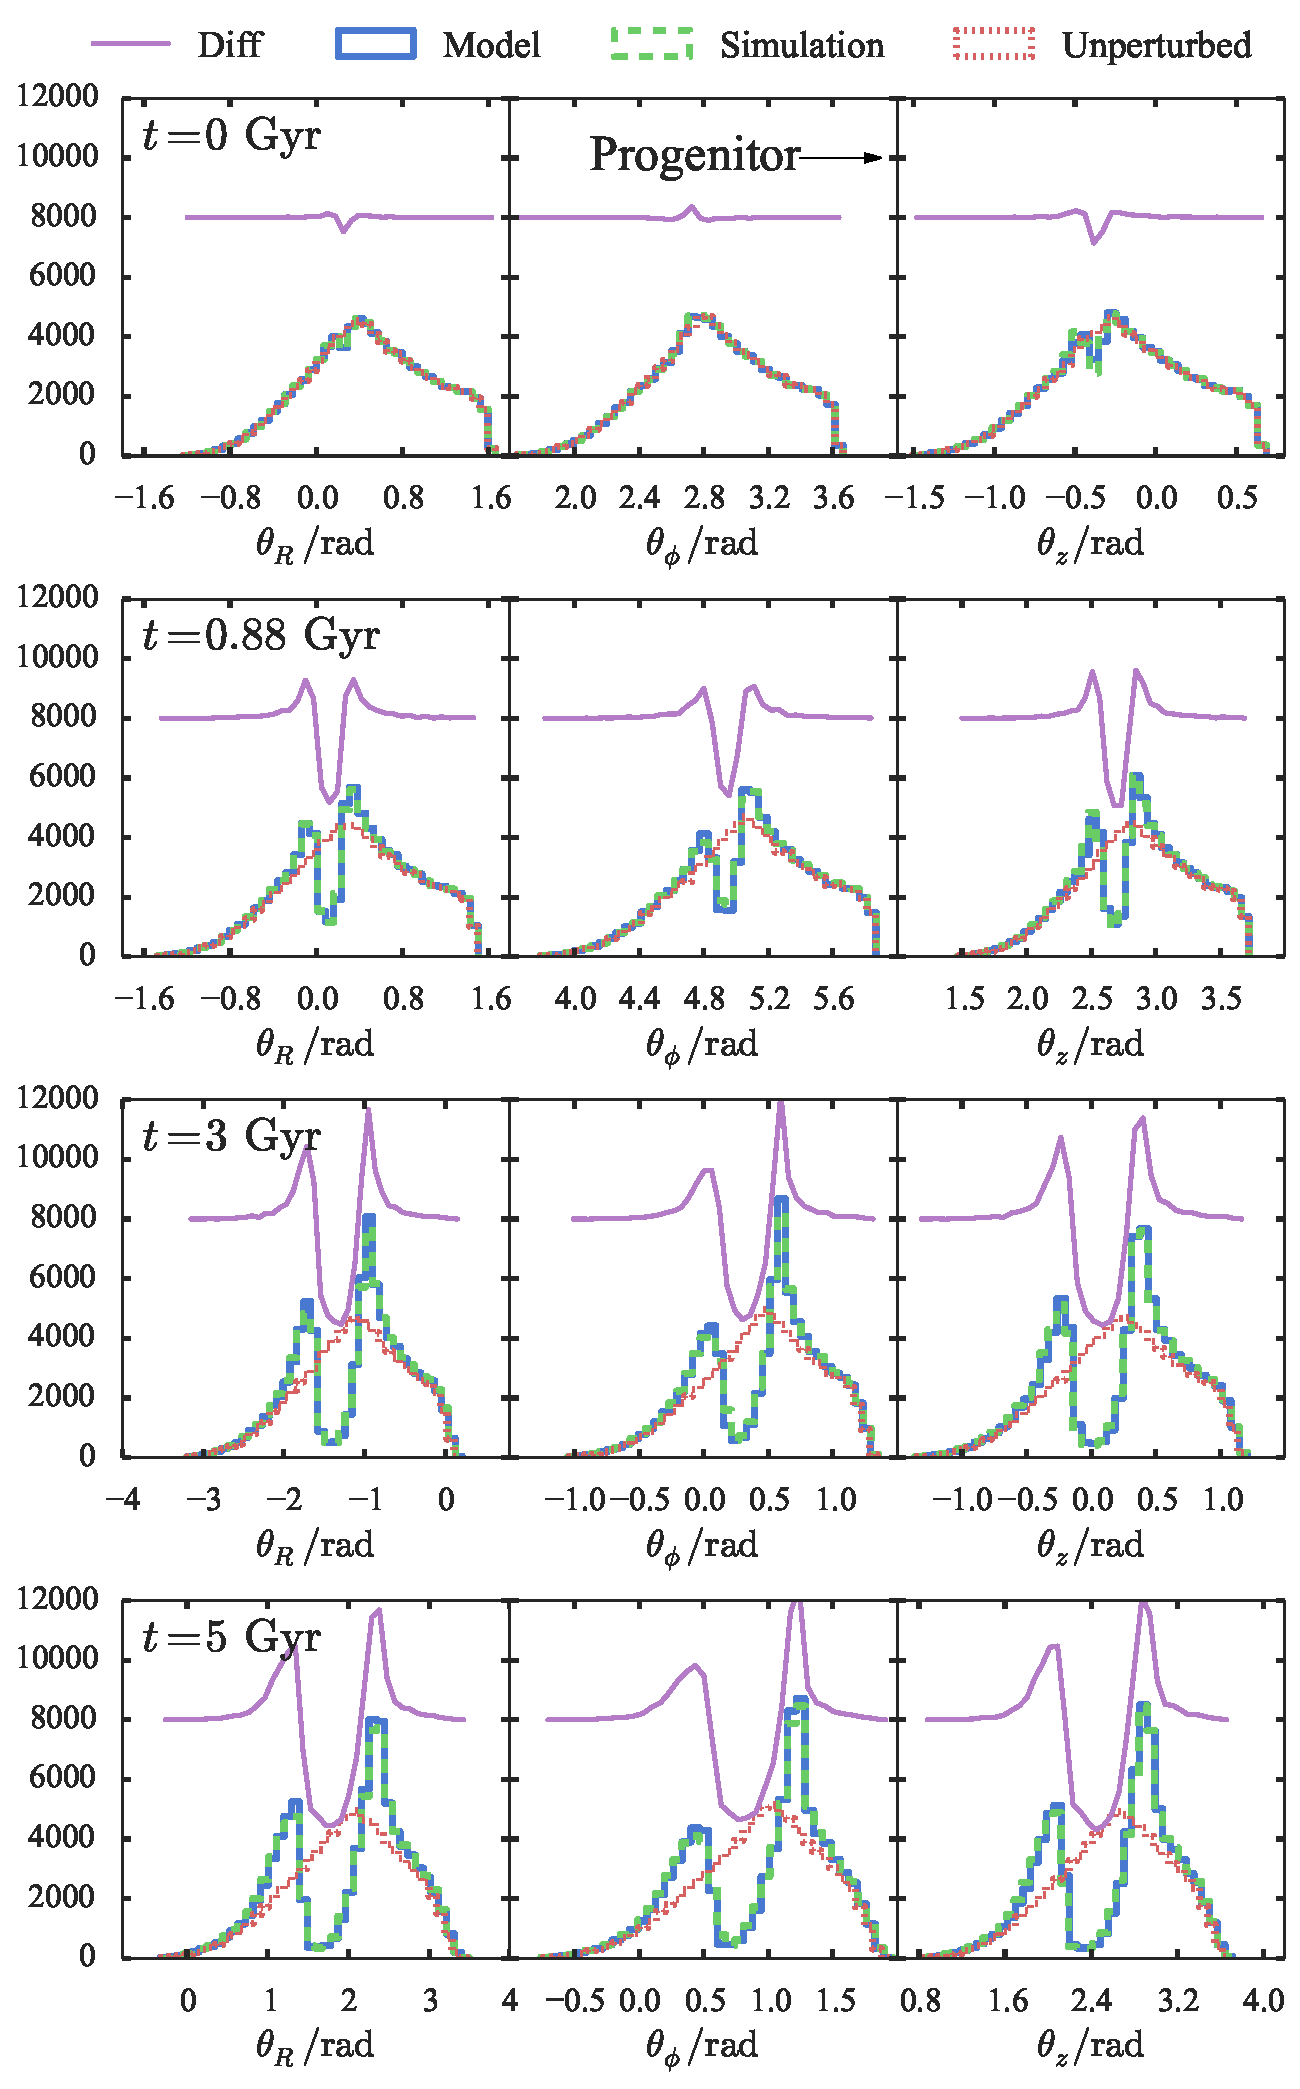
\includegraphics[width=\columnwidth]{ang_later_times}$$
\caption{
Unperturbed, perturbed and model stream for the $J_z\neq0$ progenitor. The red histograms show the unperturbed stream, the green show the perturbed stream and the blue show the unperturbed stream kicked in angle and frequency space and evolved. The purple line shows the difference between the perturbed and unperturbed streams offset by some arbitrary amount. The four rows show $0,0.88,3$ and $5\Gyr$ after impact.
}
\end{figure}

\subsection{Analytic approximations}
We now develop some understanding of the magnitude of the angle, frequency and action kicks.

For scale-free potentials of the form $\Phi\propto r^\alpha$ the Hamiltonian in action-space is well approximated by
\begin{equation}
H(\bs{J}) \propto (J_R+B(L_z+J_z/q))^\beta,
\end{equation}
where $\beta=2\alpha/(2+\alpha)$ and $B$ is a constant. In these potentials the frequencies are solely functions of the Hamiltonian so we find that
\begin{equation}
\frac{\delta\Omega_i^g}{\Omega_i}=\frac{\beta-1}{\beta}\frac{\delta H}{H}.
\end{equation}
Note in the case of the harmonic oscillator $\beta=1$ and the right-hand side vanishes as the frequencies are energy independent. The analogous approximate expression for the Hamiltonian in the scale-free logarithmic potential is
\begin{equation}
H(\bs{J}) = V_c^2\log(J_R+B(L_z+J_z/q)),
\end{equation}
such that
\begin{equation}
\frac{\delta\Omega_i^g}{\Omega_i}=-\frac{\delta H}{V_c^2}.
\end{equation}
In the case of a sub-halo flyby $\delta H=\bs{v}\cdot\delta\bs{v}$. We plot this approximation in Fig.~\ref{analytic_freq} for the case of the non-zero-$J_z$ stream.
\begin{figure}
$$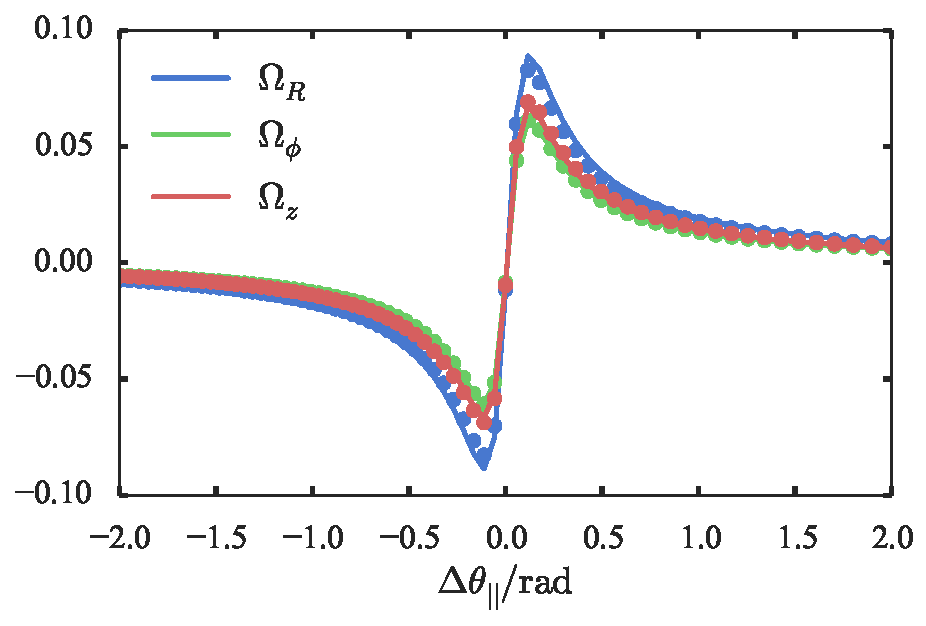
\includegraphics[width=\columnwidth]{analytic_freq}$$
\caption{
Analytic frequency kick approximation.
}
\label{analytic_freq}
\end{figure}

We would like to find analogous expressions for the actions and angles. We approximate the changes in the angles as
\begin{equation}
\begin{split}
\delta J_R \approx \frac{\delta H - \delta L \Omega_\phi}{\Omega_R},\\
\delta L_z \approx (\bs{r}\times\delta\bs{v})_z,\\
\delta J_z \approx \frac{v_z \delta v_z}{\Omega_z},
\end{split}
\end{equation}
where $\delta L = \bs{L}\cdot\delta\bs{L}/|\bs{L}|$ the change in the angular momentum. The change in $J_R$ comes from the spherical approximation and the change in $J_z$ from the assumption that it is a harmonic oscillator in the $z$ direction. These aren't great approximations but work OK (see Fig.~\ref{aa_z} and~\ref{aa_nz}).

\begin{figure}
$$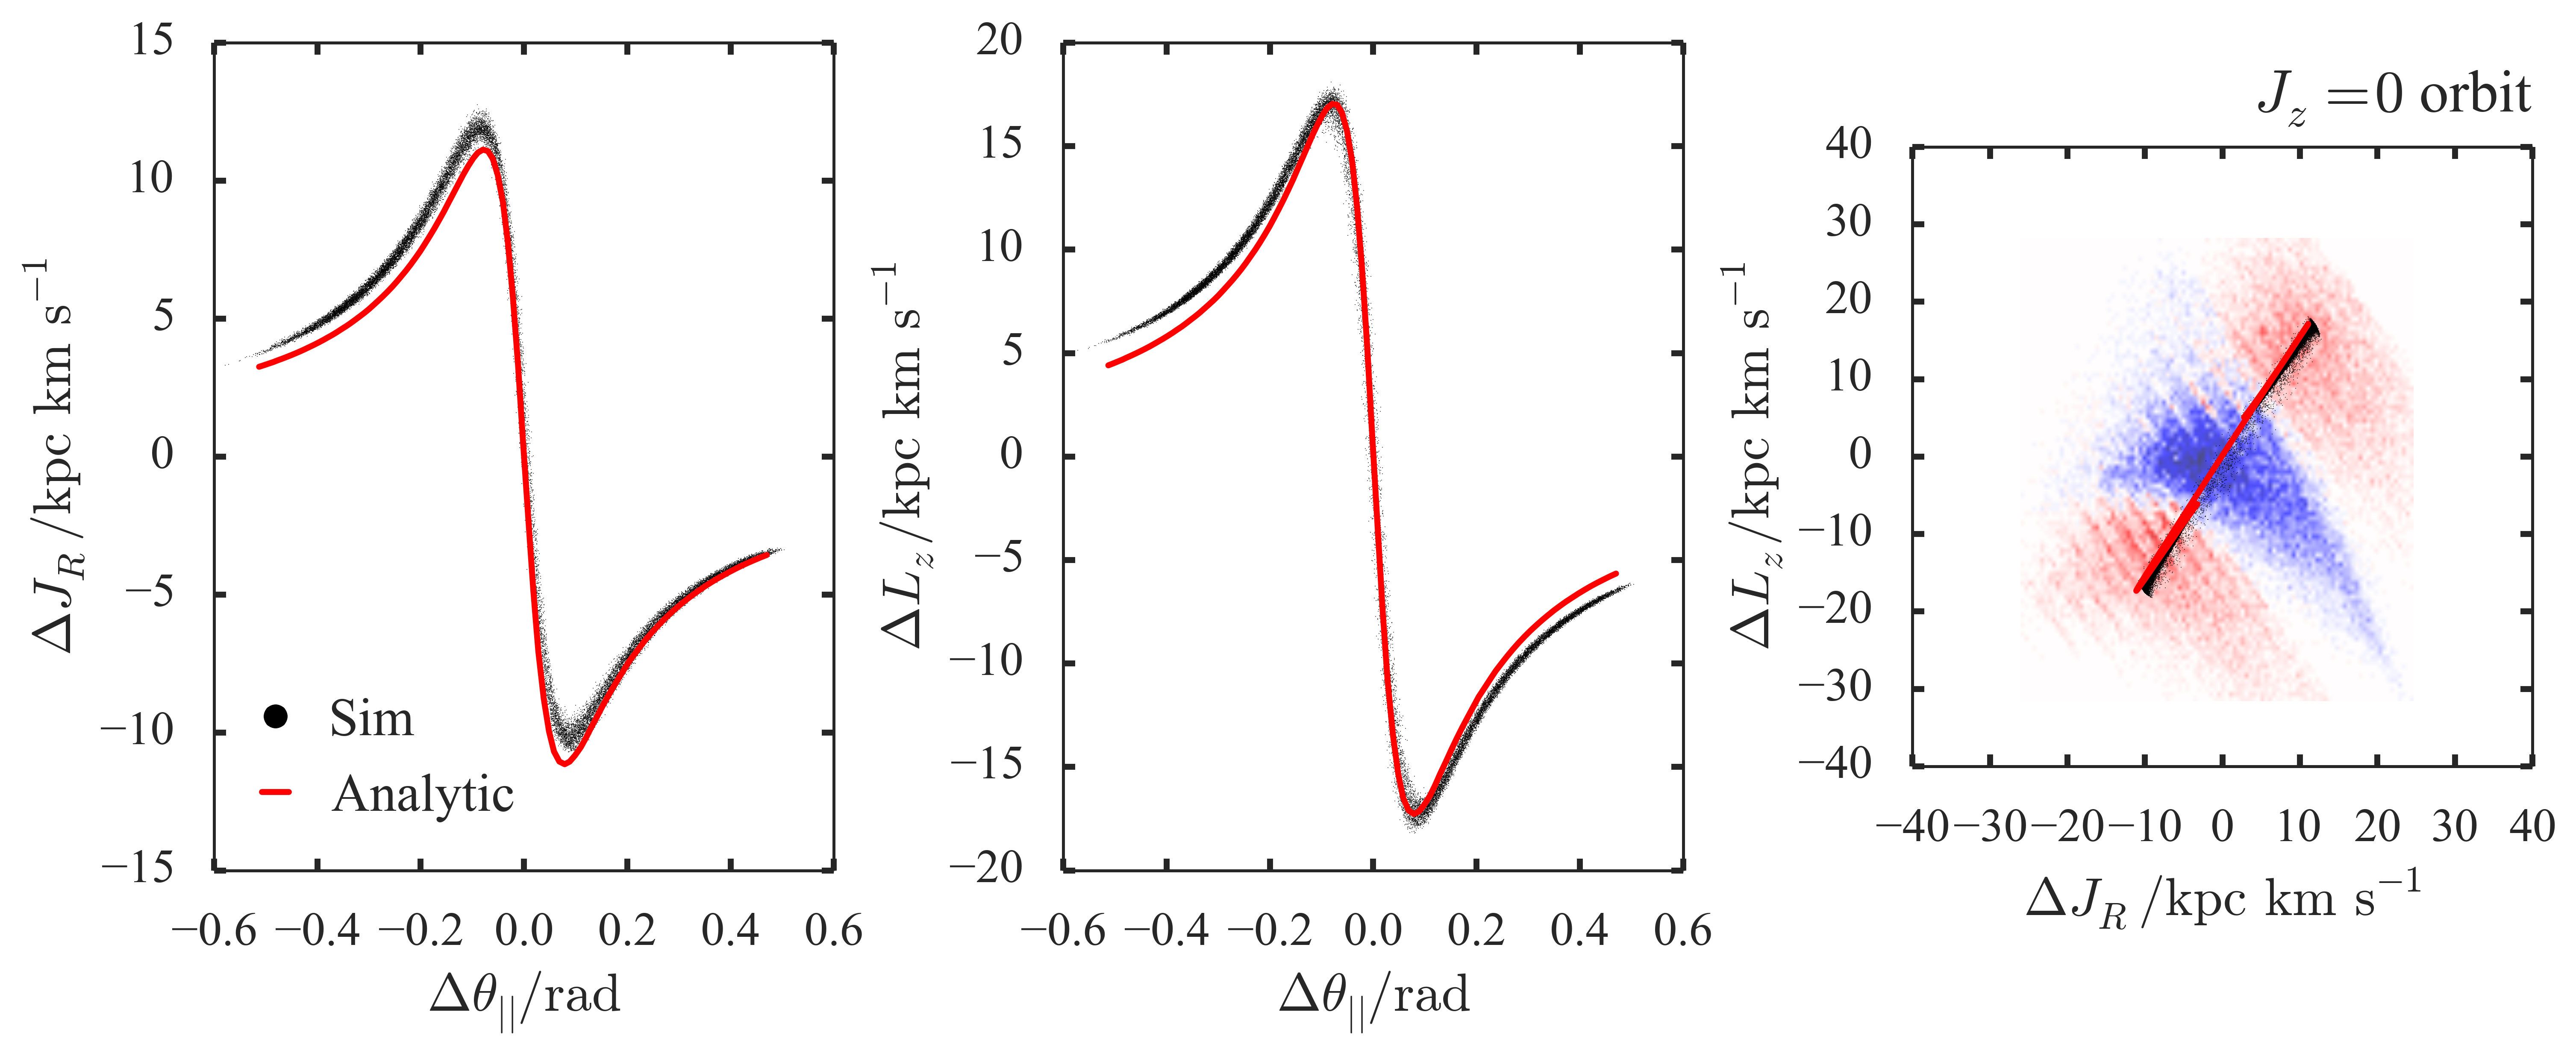
\includegraphics[width=\columnwidth]{analytic_action}$$
\caption{
Analytic action kick approximation.
}
\label{aa_z}
\end{figure}
\begin{figure}
$$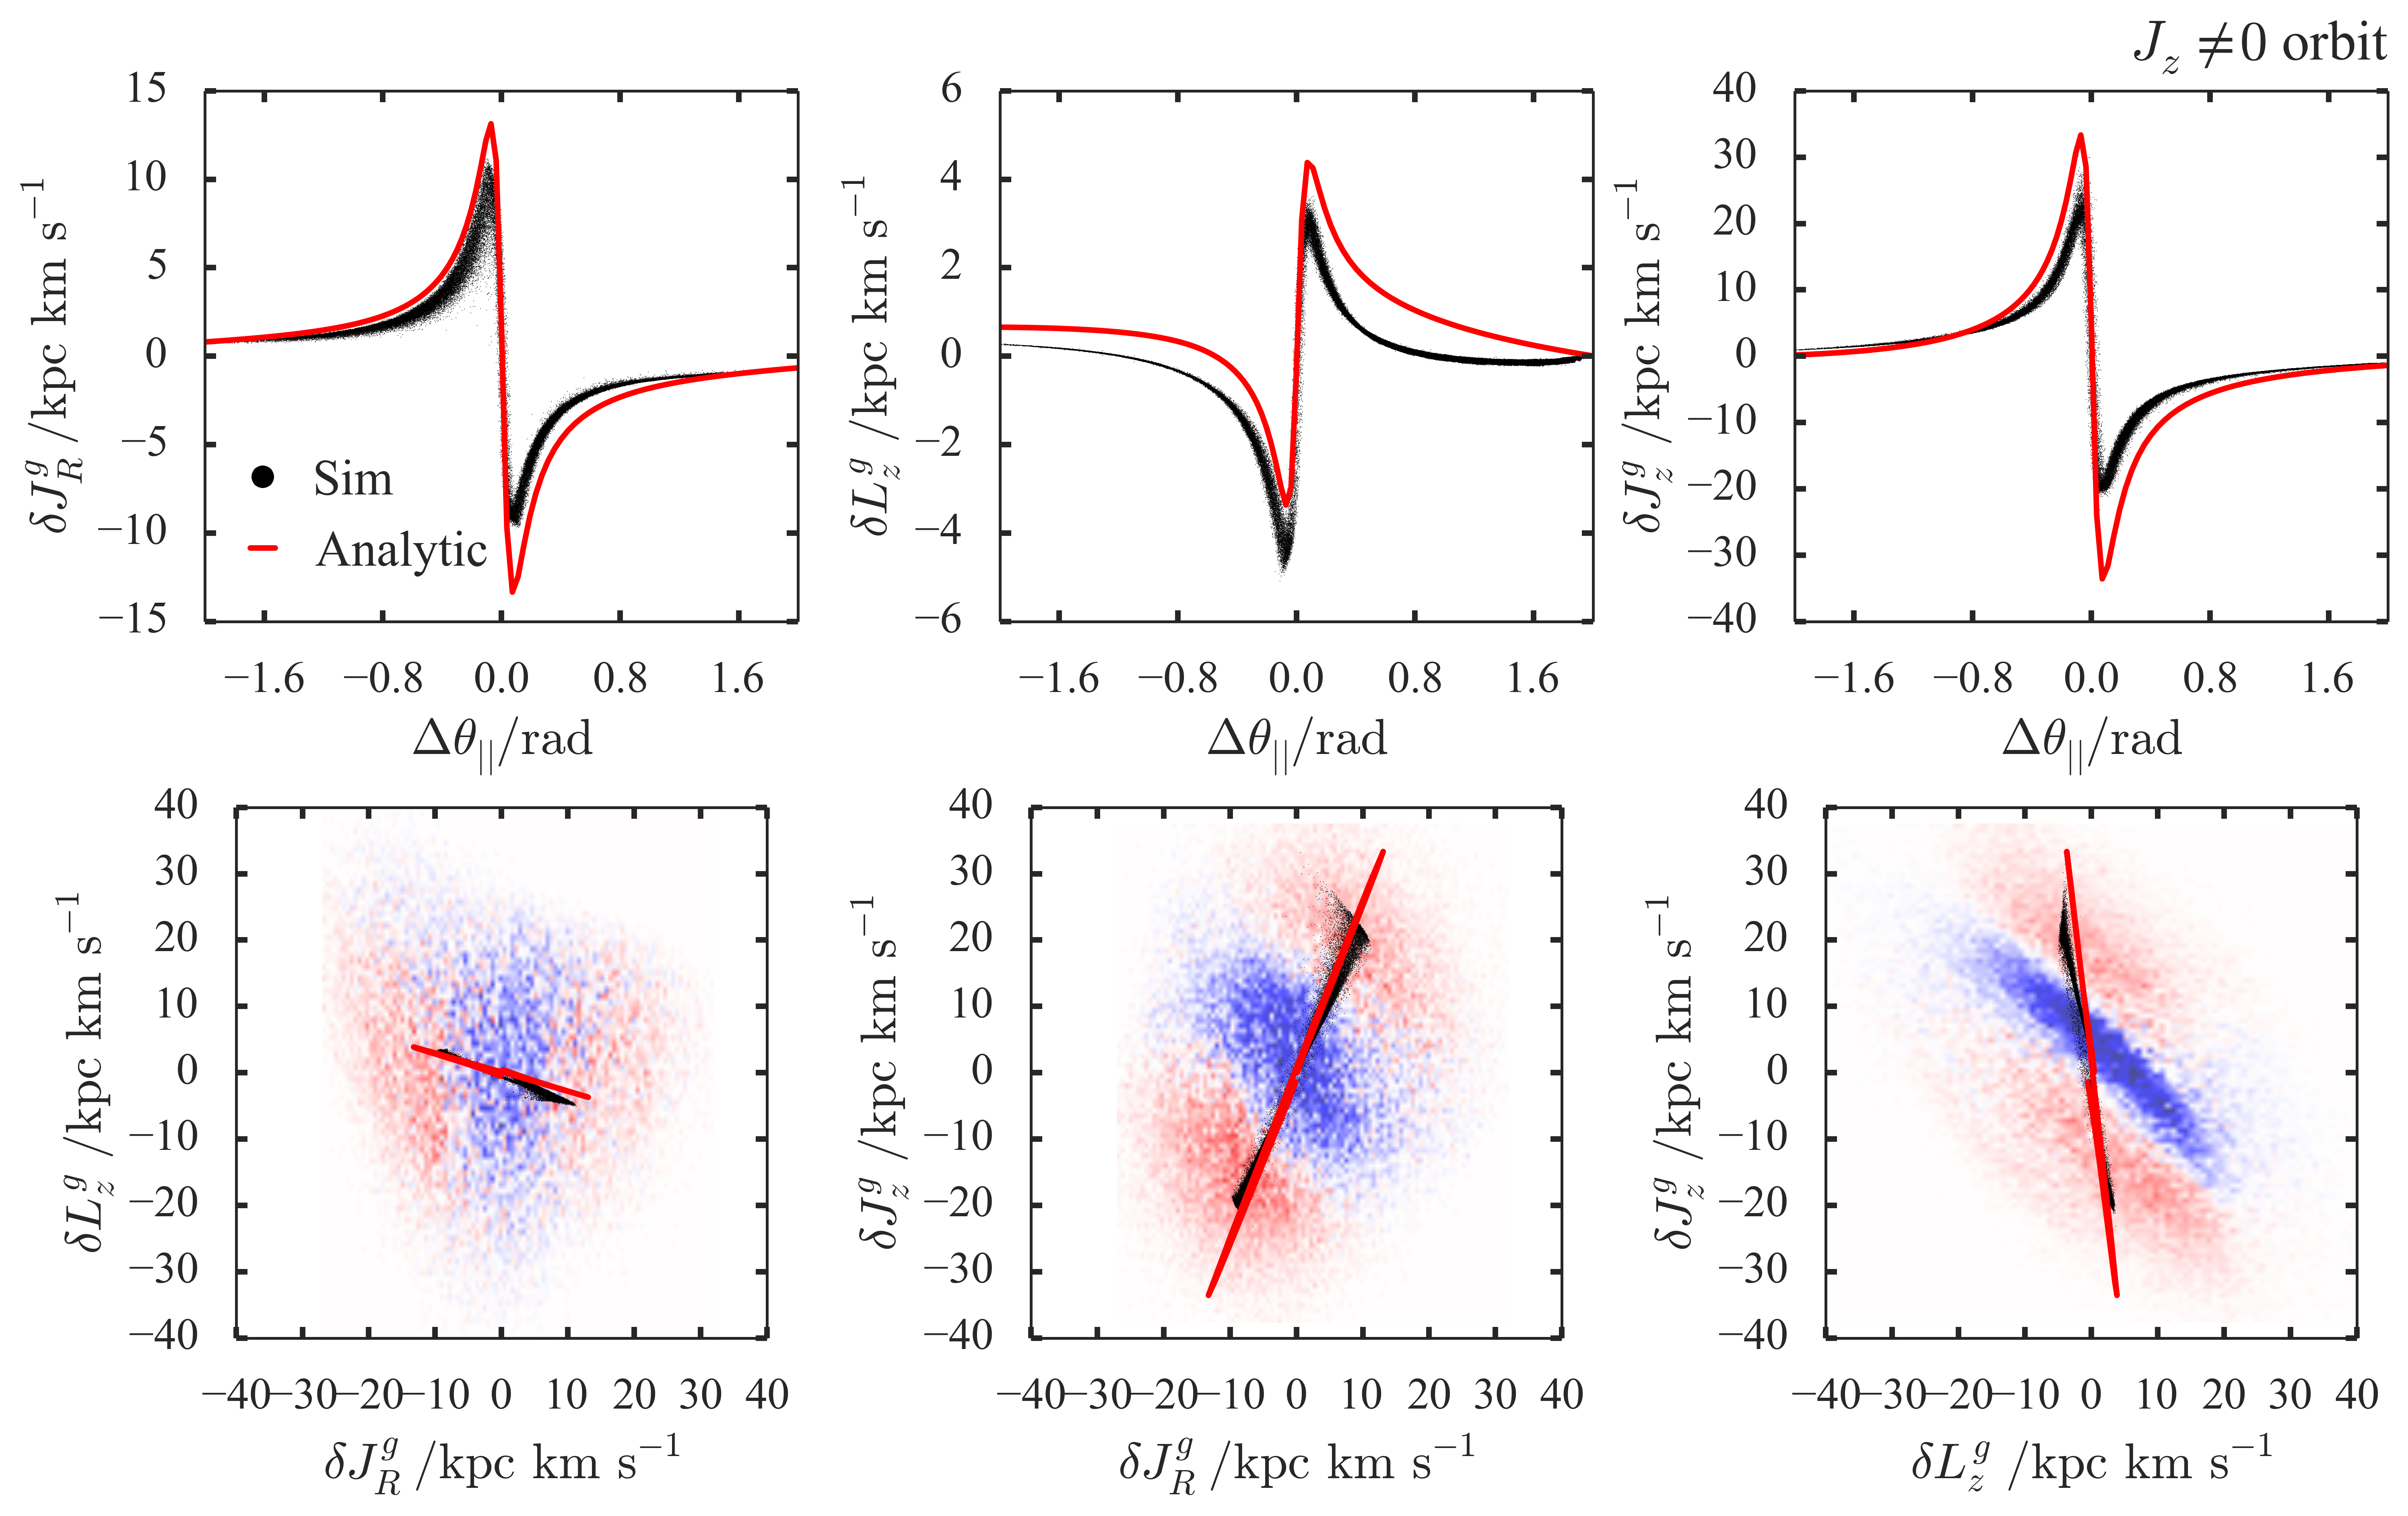
\includegraphics[width=\columnwidth]{tilted_analytic_action}$$
\caption{
Analytic action kick approximation.
}
\label{aa_nz}
\end{figure}

\subsection{Stages of stream growth}
\cite{ErkalBelokurov2015} discussed the three phases of stream gap formation in the limit that the stream progenitor is on a circular orbit. They found that on short time-scales (less than a radial period) an overdensity formed as the particles were scattered onto epicyclic orbits that brought them towards the gap centre. This was dubbed the compression phase. After a radial period the stream enters an expansion phase where the gap begins growing until the perturbed material starts to overtake unperturbed material and a caustic forms. During the expansion phase the stream gap grows linearly in time whilst during the caustic phase the growth rate slows to $t^{1/2}$. In this section we investigate and discuss how this picture relates to the formalism presented here.

\begin{figure}
% $$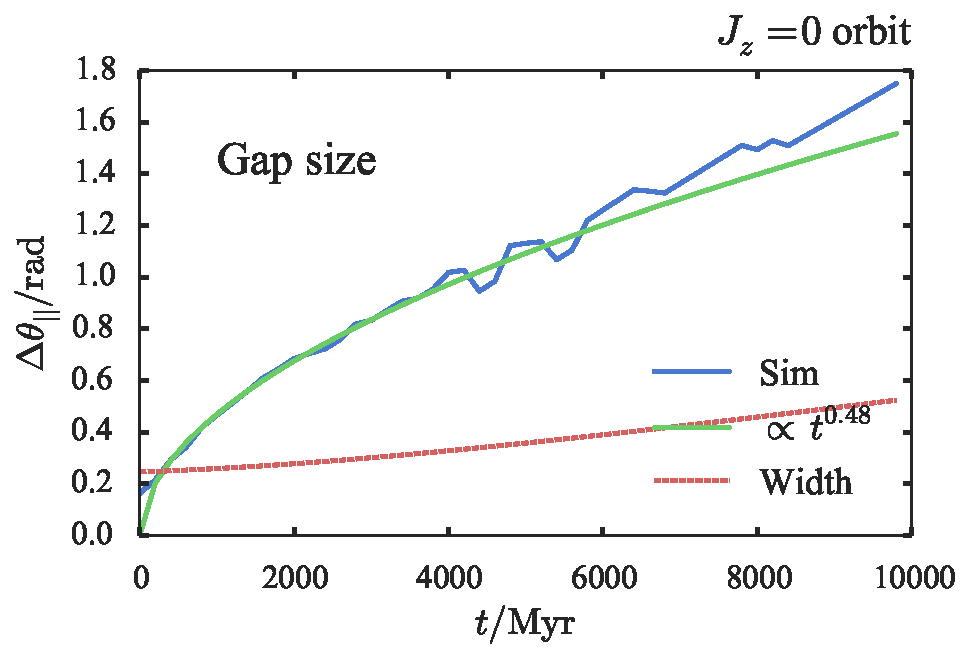
\includegraphics[width=\columnwidth]{gap_size_planar}$$
$$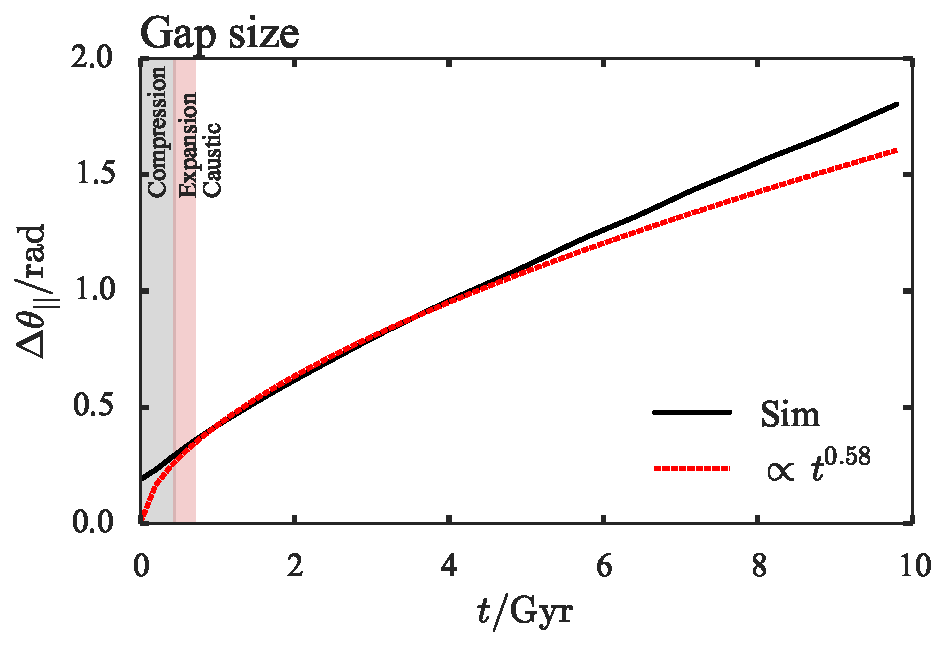
\includegraphics[width=\columnwidth]{tilted_gap_size}$$
\caption{
Gap size in angle as a function of time. Top is $J_z=0$.
}
\label{gap_size}
\end{figure}

In Fig.~\ref{gap_size} we plot the size of the gap in parallel angles as a function of time for the non-zero $J_z$ stream. This is defined as the difference between the parallel angles of the points where the perturbed and unperturbed densities are equal. We also show a best-fit line polynomial line ($\Delta\theta_{||}\propto t^n$) for the segment $t<5\Gyr$ as well as the time-scales for the different stages of gap growth. We note that there is a gap in parallel angle at $t=0$. This does not correspond to a spatial gap but is due to the angle kicks from the sub-halo that have shifted the stars to slightly different orbital phases. This initial angle kick appears to dominate on a time-scale of $\sim400\Myr$ after which the best-fit polynomial is a much better match. This also appears to correlate with the end of the compression phase. Therefore, it seems that the compression phase is associated with the initial angle kicks. We can understand this by considering a simple example of a stream on a radial orbit. Here the parallel angle is purely the radial angle. The shape of the angle kicks will be very similar to those in Fig.~\ref{kicks_nzero} with the angles in front of the gap given a positive kick and those behind given a negative kick. At a fixed position increasing the radial angle means we are now closer to apocentre so the apocentre has moved inwards and the particle must move more slowly. Likewise decreasing the radial angle moves apocentre further out and the particle must move faster. Therefore, the particles behind the gap move faster than those in front and an overdensity forms.

We use the formulae from \cite{ErkalBelokurov2015} to calculate the time-scale on which the caustic begins to form. In this case the expansion phase is very short and so the subsequent evolution should go with the square-root of time. We see, however, that this is only approximately true up to $\sim4\Gyr$ after which the growth rate is faster than this. We will return to this point later and only mention here that it is due to the gap forming on an already growing underlying stream.

Our discussion has related to the size of the gap in parallel angle. Whilst this is an appropriate space for understanding general stream morphology it is awkward to see the relationship with the observed stream properties. We briefly investigate this by projecting the model back into real-space. For this purpose we use the publicly-available torus code from \cite{McMillanBinneyDehnen2015}. We construct eight tori on the corners of an action-space box that encompasses the full perturbed distributions and interpolate the frequencies to find the actions of the perturbed particles. We then interpolate the Fourier coefficients of the tori in action-space to construct a torus of the required actions for each particle and request the $(\bs{x},\bs{v})$ corresponding to the angles of the particle. We then find a plane that minimises the perpendicular spread of the stream and compute the size of the gap in the azimuthal angle in the plane in the same way as in parallel angle space. We plot both the azimuthal gap size and the parallel angle gap size as a function of time in Fig.~\ref{real_v_angle}. As expected the azimuthal gap size oscillates but it is well enveloped by the parallel angle gap size and it appears that the average azimuthal gap size well correlates with the parallel angle gap size. We also plot the minimum and maximum density contrasts (defined as perturbed divided by unperturbed density). The azimuthal density contrast oscillates about the parallel angle density contrast. We also can clearly see the gap forms immediately in parallel angle whilst in azimuthal angle there is a small peak due to the compression phase.

\begin{figure}
$$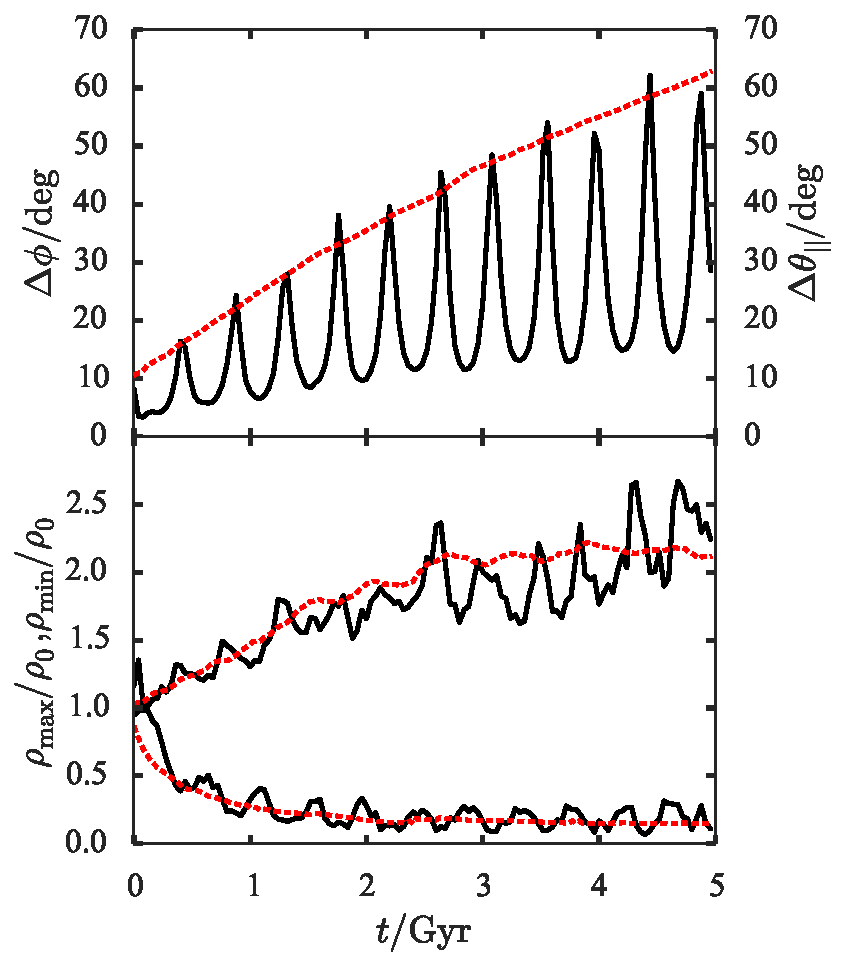
\includegraphics[width=\columnwidth]{real_vs_angle_properties}$$
\caption{
Gap properties in real and angle space. In the top panel we show the gap size in the azimuthal angle of a plane fitted through the stream in solid black and the gap size in parallel angle in dashed red. In the bottom panel we show the minimum and maximum density contrast in these two spaces.
}
\label{real_v_angle}
\end{figure}

\section{Varying the impact properties}
We have demonstrated that we are able to adequately model the impact of a sub-halo on a stream and the subsequent evolution. With this machinery in place we are able to rapidly simulate the effects of any sub-halo fly-by. In this section we will discuss the differences in the subsequent stream structure as a function of the sub-halo mass and the sub-halo impact location. We repeat the exercise performed in Section~\ref{section::simulation} of simulating the sub-halo fly-by on a simulated unperturbed stream and inspecting the subsequent evolution.

\subsection{Varying the sub-halo mass}
First, we investigate the properties of the stream as a function of sub-halo mass. We adopt the scaling relation between the mass and scale radius of the sub-halo Plummer sphere of
\begin{equation}
M\propto r_s^{2.5}.
\end{equation}
Keeping all other properties of the sub-halo fly-by the same we simulate the effects of a $10^7M_\odot$ and $10^{7.5}M_\odot$ sub-halo. In Figure~\ref{varying_mass} we show the gap after $t=880\Myr$, the gap size as a function of time and the minimum and maximum density contrast as a function of time. As expected the gap size is deepest and grows fastest for the highest mass sub-halo. In all cases the minimum density contrast plateaus in time.

\begin{figure*}
% $$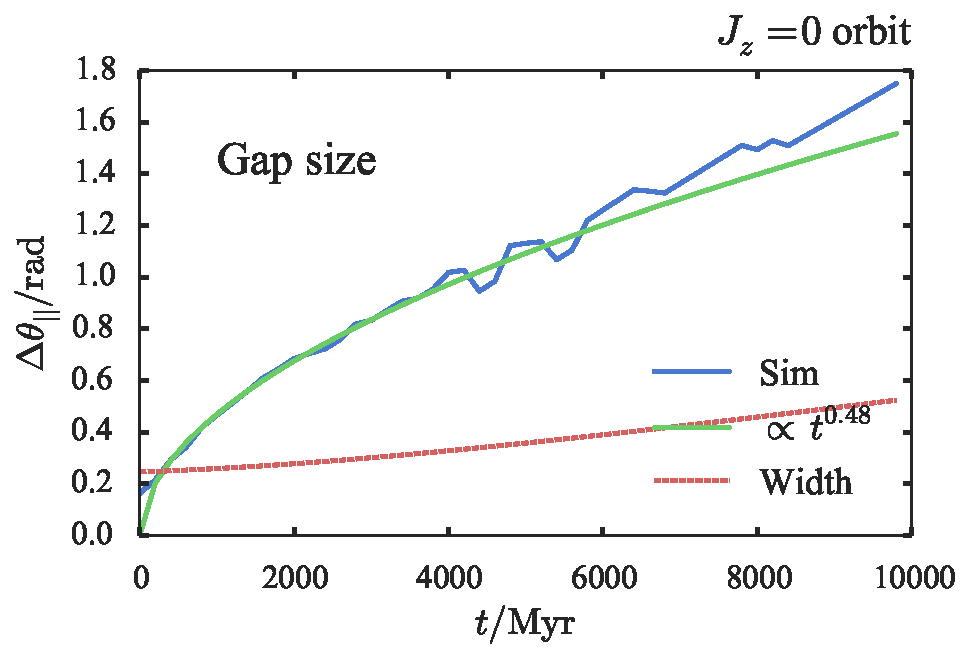
\includegraphics[width=\columnwidth]{gap_size_planar}$$
$$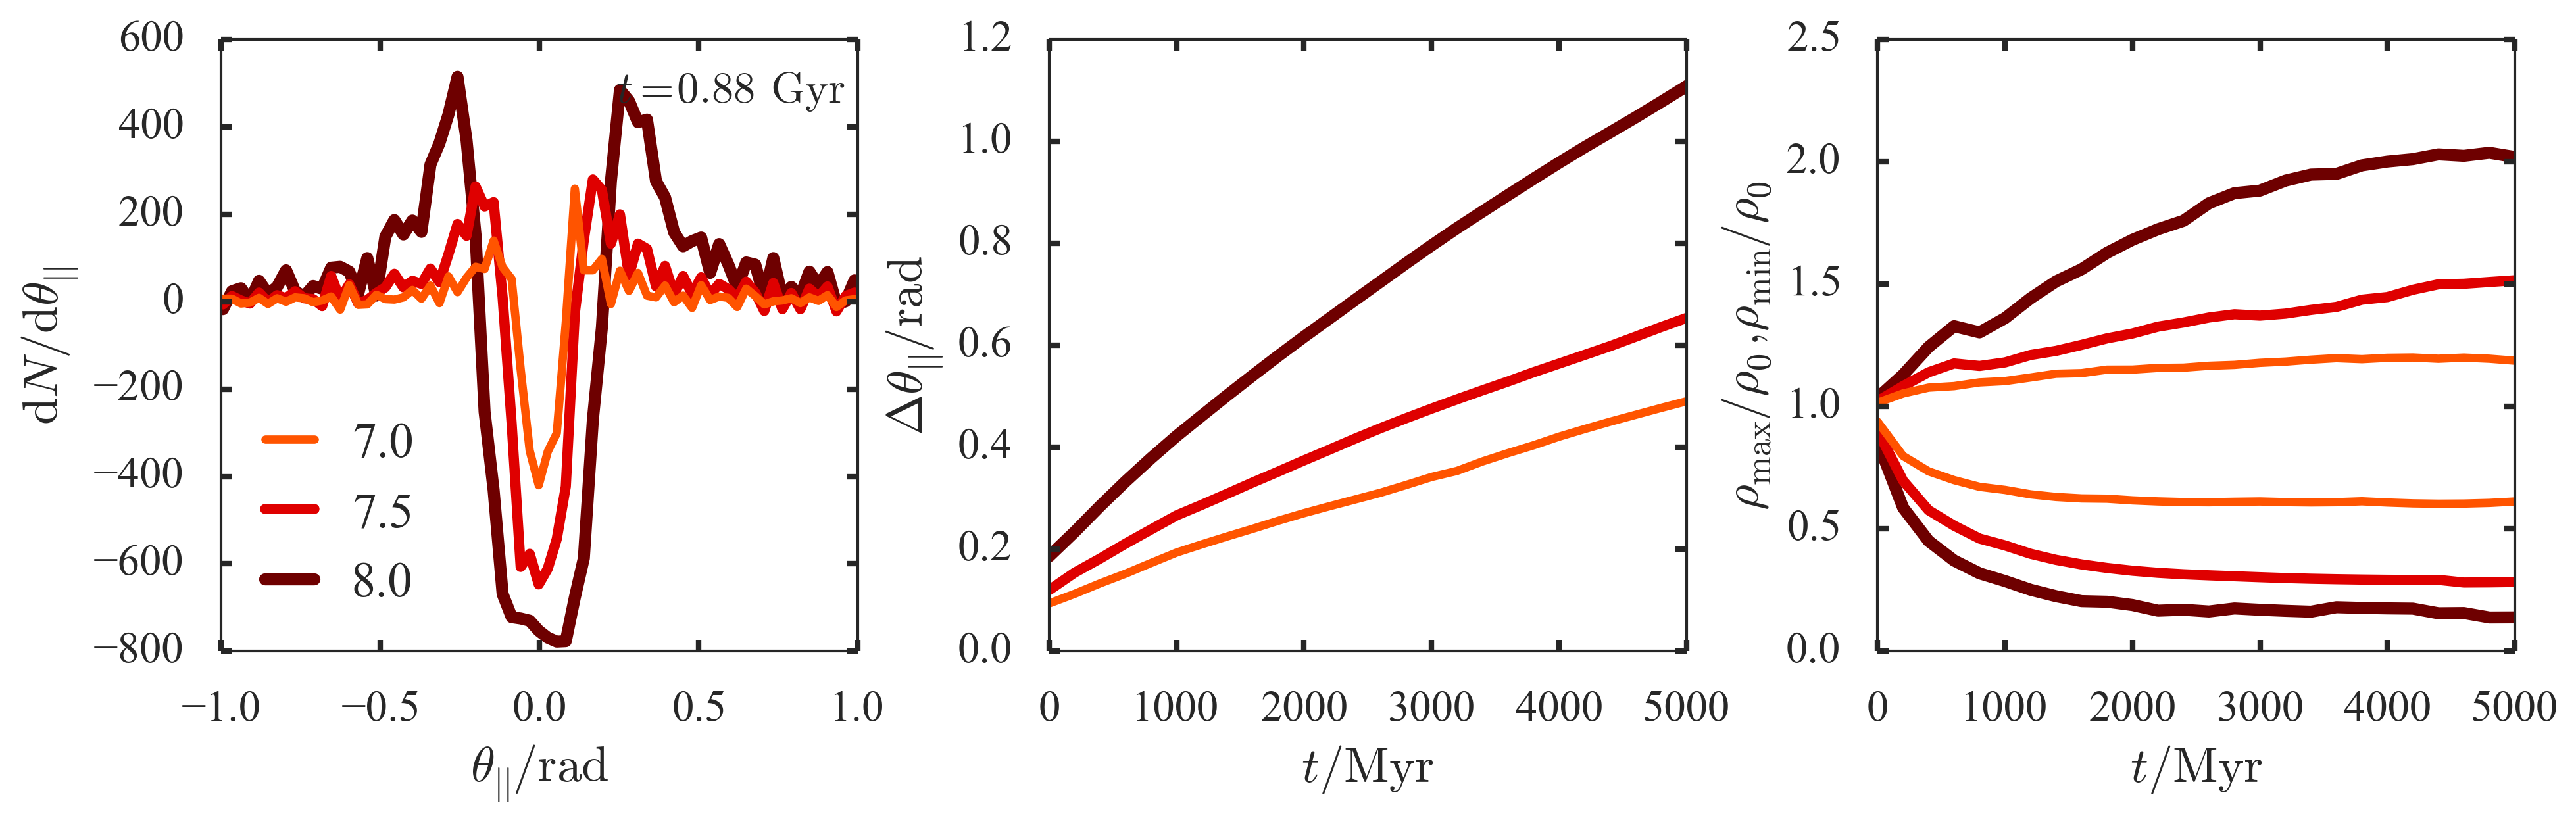
\includegraphics[width=\textwidth]{different_masses}$$
\caption{
Properties of the stream as a function of sub-halo mass. The thick brown line corresponds to $10^8M_\odot$, the medium red line $10^{7.5}M_\odot$ and the thin orange line $10^7M_\odot$. The left panel shows the difference between the perturbed and unperturbed simulations in parallel angle after $t=880\Myr$, the middle panel shows the gap size as a function of time and the right panel shows the minimum and maximum density contrast as a function of time.
}
\label{varying_mass}
\end{figure*}
\subsection{Varying the impact geometry}
Now we investigate how the stream changes as a function of where along the stream the impact occurs. In addition to the inspected geometry of Section~\ref{section::simulation} we simulate an impact closer to the progenitor ($[x,y,z]=[-15.3,-9.8,9.3]\,\mathrm{kpc},[v_x,v_y,v_z]=[41.9,-183.0,152.2]\,\mathrm{km\,s}^{-1}$) and one further from the progenitor ($[x,y,z]=[-1.2,12.9,-10.8]\,\mathrm{kpc},\,[v_x,v_y,v_z]=[-239.8,-100.6,87.0]\,\mathrm{km\,s}^{-1}$). Again, we fix all other parameters of the impact to those in the original simulation, including the absolute velocity of the sub-halo. In Fig.~\ref{varying_geometry} we plot the locations of these impacts in both real-space ($ the (x,y)$ plane) and in parallel angles. The near impact is in the regime where the mean parallel frequency is approximately constant with the parallel angle whilst the far impact is in the regime where the mean frequency is decreasing linearly with the parallel angle. In this far regime the stream is well ordered in energies, whilst in the near regime the stream particles have not had sufficient time to order themselves by energy. We plot the difference between the perturbed and unperturbed simulations in parallel angle for two times. The density contrast at the large negative parallel angle for the far case is very large at late times as the number density in the unperturbed simulation at these large separations is low. A similar effect is seen at large positive parallel angle for the near case but here it should be noted that we have not included the effect of more stars entering the stream as they are stripped from the progenitor. In the lower panels we show the gap size and the minimum/maximum density contrast as a function of time. The gap size in all three cases is very similar for $t<3\Gyr$ but they diverge at larger times as the far impact gap size increases faster than the near impact. We can understand this as in the far case the gap is forming on an already growing stream as the underlying stream structure is well ordered. However, in the near case the stream is mixed so the underlying stream is growing more slowly. In all cases the minimum density plateaus to a similar value.

\begin{figure}
% $$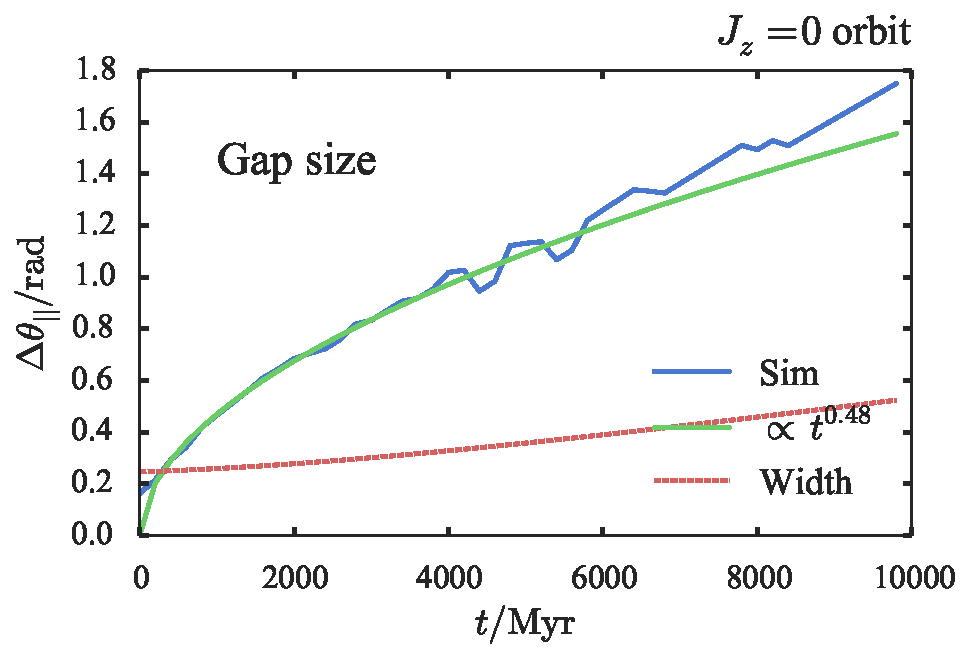
\includegraphics[width=\columnwidth]{gap_size_planar}$$
$$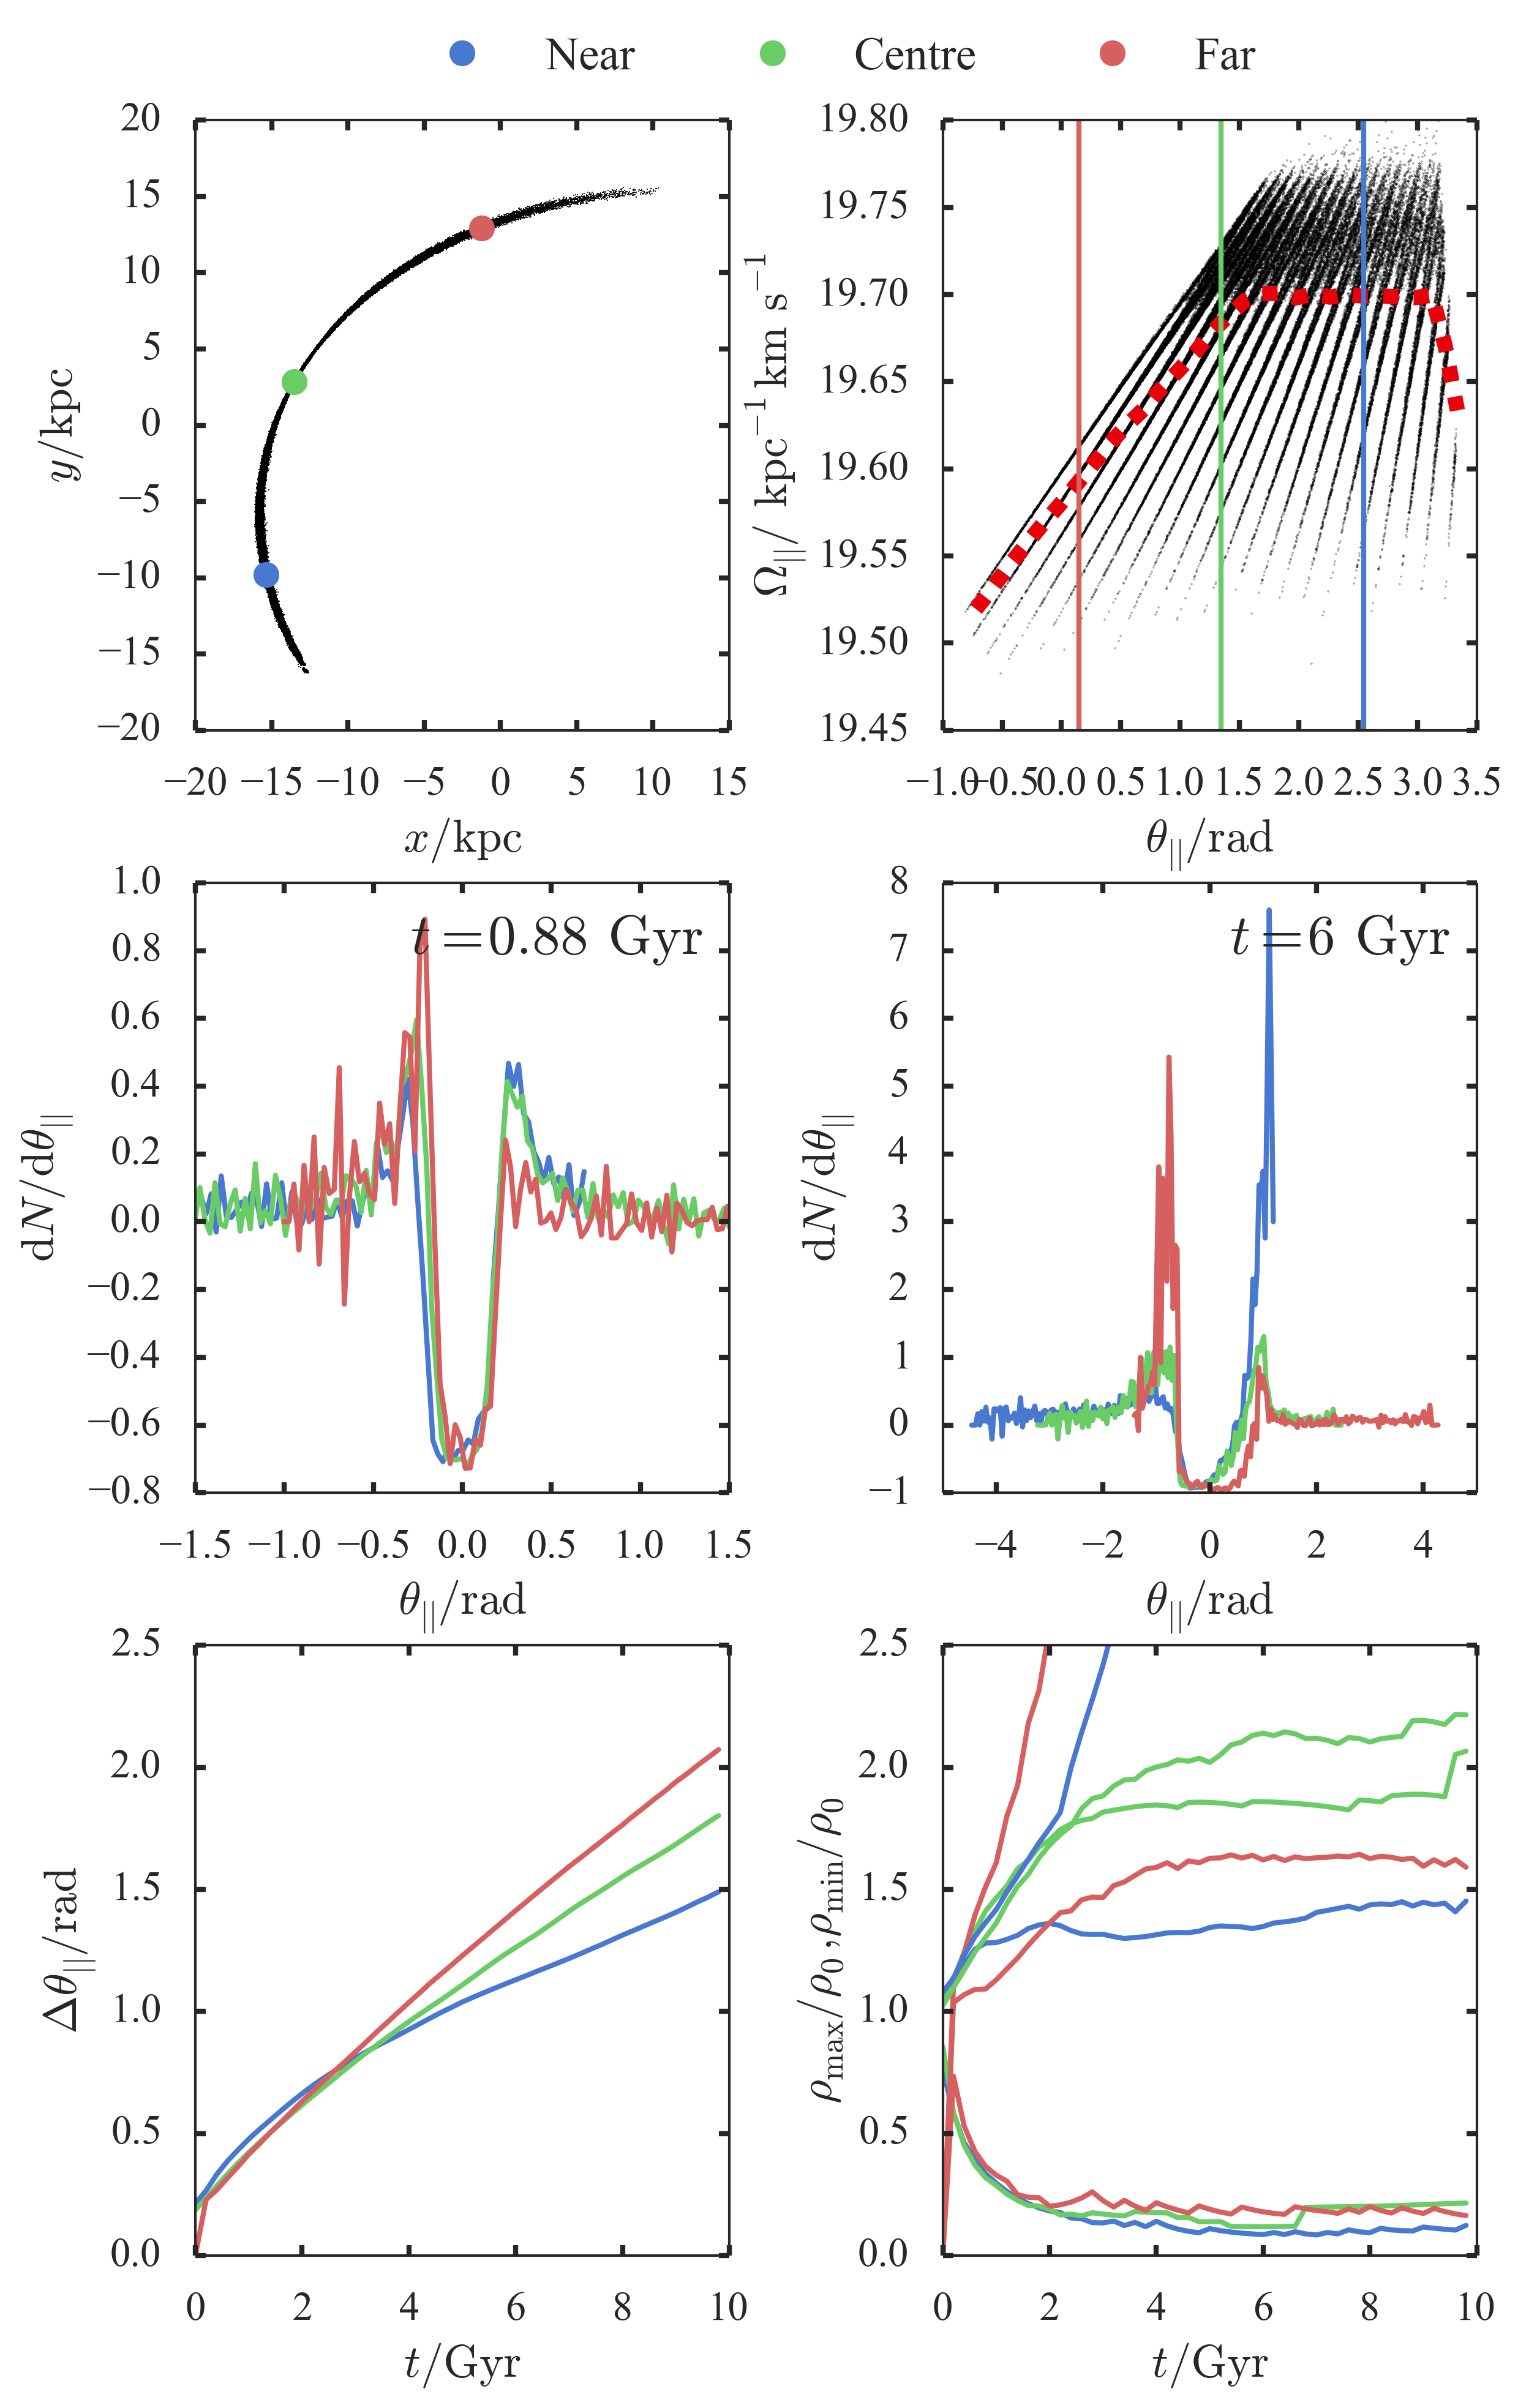
\includegraphics[width=\columnwidth]{different_strike_points}$$
\caption{
Properties of the stream as a function of sub-halo mass. The thick brown line corresponds to $10^8M_\odot$, the medium red line $10^{7.5}M_\odot$ and the thin orange line $10^7M_\odot$. The left panel shows the difference between the perturbed and unperturbed simulations in parallel angle after $t=880\Myr$, the middle panel shows the gap size as a function of time and the right panel shows the minimum and maximum density contrast as a function of time.
}
\label{varying_geometry}
\end{figure}

\section{Discussion}
\begin{enumerate}
\item What doesn't our model encompass?
\item What other sources of substructure are there?
\item Could one use this as a way to identify a gap (matched filter) or do we only bring in the big guns after the gap has been found?
\item Many smaller subhaloes?
\end{enumerate}

\section{Conclusions}


\section*{Appendix}
\subsection{Accuracy of angle, frequency and action computation}
We use the method of \cite{SandersBinney2014} to compute the actions, angles and frequencies. In this appendix we present some checks of the accuracy of the action, angle and frequency calculation as well as estimates of the errors in these quantities. In Fig.~\ref{SingleOrbitCheck} we plot the variation in the actions and frequencies as a function of time for a single orbit integrated for a long time. The errors in the actions are $\sim0.04\kpc\kms$ and the errors in the frequencies are $\sim10^{-4}\kpc^{-1}\kms$. We also plot the difference in the angles calculated at each time-step and those found from calculating $\theta_0+\Omega t$. The shaded regions shows the lines $\theta(t=0)+(\Omega\pm\Delta\Omega)t$ so there is some residual noise from the angle calculation. We subtract off the linear component to find an estimate of the error in the angles of $\sim10^{-3}\rad$. In conclusion we are satisfied that our action, frequency and angle calculation accuracy is resolving the features of the gap and stream.

\begin{figure}
$$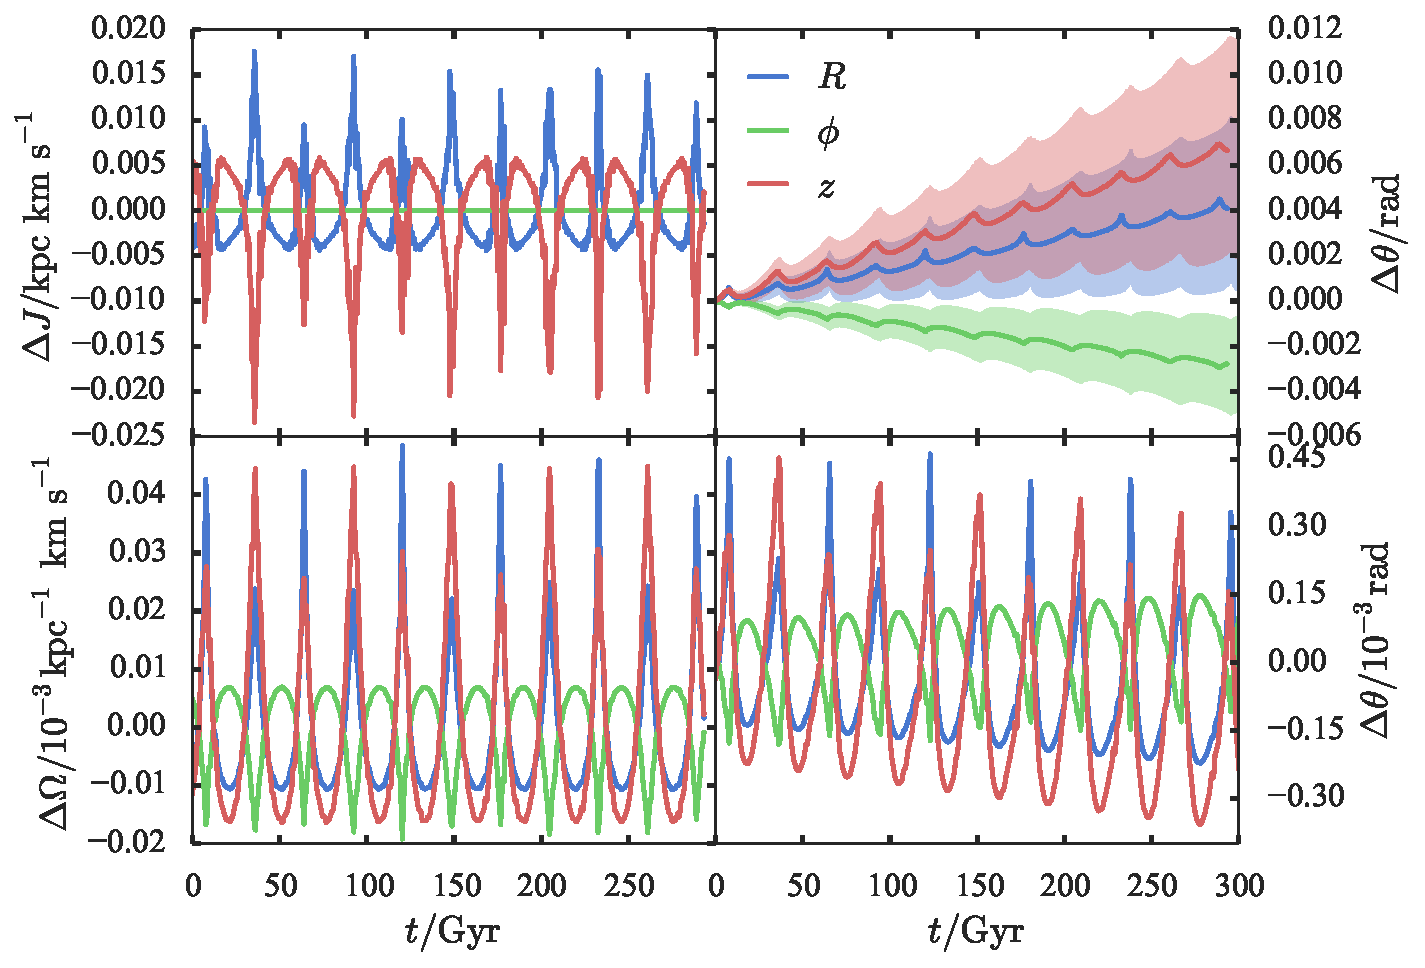
\includegraphics[width=\columnwidth]{action_error}$$
\caption{Errors in the actions, frequencies and angles for a single orbit: the left panels show the deviation of the actions and frequencies as a function of time for a single particle taken from the simulation. The top right panel shows the difference in the angle coordinate from the value calculated using $\theta(t=0)+\Omega t$ and the bottom right panel shows the top right panel with the linear component extracted so is an estimate of the error in the angles.}
\label{SingleOrbitCheck}
\end{figure}

Another check is to evolve the simulation snapshot forward in angles and frequencies and compare the angle distribution at a later time with the angle distribution calculated from a later snapshot. We plot the histogram of the differences in the angle distributions in Fig.~\ref{TwoSnapshotCheck}. This also indicates that the error in the angle calculation is $\sim10^{-3}\rad$.

\begin{figure}
$$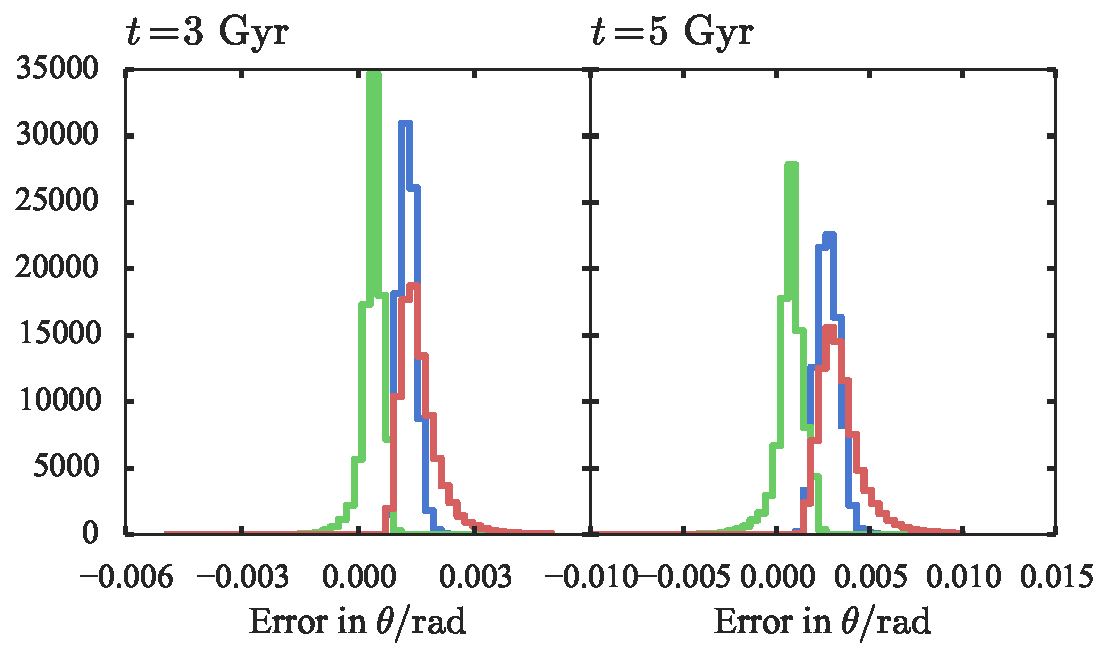
\includegraphics[width=\columnwidth]{ang_error}$$
\caption{Errors in the angles: histograms of the angle difference between the angles found from evolving the $880\Myr$ snapshot and those found from re-calculating the angles at the later time. The left panel shows the difference at $3\Gyr$ and the right at $5\Gyr$. Note the growth in the error with time as the errors in the frequencies are compounded with time.}
\label{TwoSnapshotCheck}
\end{figure}


\label{lastpage}
\end{document}



% \section{Stream model}
% The dynamical stream models in Sanders (2014) and Bovy (2014) are expressed in angle-frequency space: $p_{\rm st}(\boldsymbol{\Omega},\btheta)$. Here the frequencies are the derivatives of the Hamiltonian with respect to the actions $\boldsymbol{\Omega} = \upartial H/\upartial \bs{J}$. The frequency distribution is a Gaussian in two directions and a double Gaussian in the third, more extended dimension. The angle distribution is calculated from the frequency distribution under the assumption of some stripping time distribution $p(t)$. If we know that a subhalo passed through at some time $t_k$ can we design a model that reflects this?

% \section{Kick model}
% Given a set of angle-actions, how do we work out the change given an external potential? One tempting thing to do is Hamiltonian perturbation theory. We can attempt to infer the change in angles and actions from some external potential. However, I feel this overcomplicates matters. Instead we just stick with the impulse approximation of Erkal \& Belokurov (2015). In this approximation the positions $\bs{x}$ of the particles do not change over the short time the external potential acts and the velocities $\bs{v}$ change instantaneously by an amount $\delta\bs{v}$. Expressions for the change in velocity are given in Erkal \& Belokurov (2015) in a coordinate system where the stream extends along one of the coordinate axes. With these expressions we can calculate the change to the angles and actions as

% \begin{equation}
% \begin{split}
% \delta \bs{J} &= \frac{\upartial \bs{J}}{\upartial \bs{v}}\Big|_{\bs{x}}\cdot \delta\bs{v},\\
% \delta \bs{\theta} &= \frac{\upartial \bs{\theta}}{\upartial \bs{v}}\Big|_{\bs{x}}\cdot \delta\bs{v}.
% \end{split}
% \end{equation}

% I tried some generating function things to see whether these derivatives could be rewritten in some informative way but to no avail.

% Now we work out the expressions for the frequencies and angles at some time $t$ where $t>t_k$. We set $t=t_0$ to be the time at which the cluster was released.

% \begin{equation}
% \begin{split}
% \boldsymbol{\Omega} &= \boldsymbol{\Omega}'+\mat{D}\cdot\frac{\upartial \bs{J}}{\upartial \bs{v}}\Big|_{\bs{x}(t_k)}\cdot\delta\bs{v}(\bs{x}(t_k)),\\
% \bs{\theta} &= \bs{\theta}'+\Big(\mat{D}\cdot\frac{\upartial \bs{J}}{\upartial \bs{v}}\Big|_{\bs{x}(t_k)}(t-t_k)+\frac{\upartial \bs{\theta}}{\upartial \bs{v}}\Big)\cdot\delta\bs{v}(\bs{x}(t_k)).
% \end{split}
% \end{equation}
% $\mat{D}$ is the Hessian matrix. The primed quantities are the angles and frequencies if no kick had occurred. Then we can still use the stream model $p_{\rm st}(\boldsymbol{\Omega},\btheta)$ but the probability is evaluated at
% \begin{equation}
% \begin{split}
% \boldsymbol{\Omega}' &= \boldsymbol{\Omega}-\mat{D}\cdot\frac{\upartial \bs{J}}{\upartial \bs{v}}\Big|_{\bs{x}(t_k)}\cdot\delta\bs{v}(\bs{x}(t_k))=\boldsymbol{\Omega}-\bs{F},\\
% \bs{\theta}' &= \bs{\theta}-\Big(\mat{D}\cdot\frac{\upartial \bs{J}}{\upartial \bs{v}}\Big|_{\bs{x}(t_k)}(t-t_k)+\frac{\upartial \bs{\theta}}{\upartial \bs{v}}\Big)\cdot\delta\bs{v}(\bs{x}(t_k)) = \bs{\theta}-\bs{G}.
% \end{split}
% \end{equation}

% I think with these expressions we can get somewhere.

% First we posit a kick time $t_k$ and work out where the progenitor was at $t=t_k$. We then select a few points labelled $i$ along the 1D stream a la Bovy (2014) and work out the $\mat{D}_i$, $\frac{\upartial \bs{J}}{\upartial \bs{v}}\Big|_{\bs{x}_i}$ and $\frac{\upartial \btheta}{\upartial \bs{v}}\Big|_{\bs{x}_i}$. We then should rotate to a frame in which the progenitor velocity is along the $y$ direction and use the relations for the kick in this frame to find the kicks at the points $i$. We then rotate the kicks back to the original frame and calculate the changes to the angles and frequencies $\bs{F}$
%  and $\bs{G}$.

% In the neighbourhood of the true stream we use the scheme of Bovy (2014) to find the linear transformation between actions, frequencies and angles and positions and velocities for a few points to construct the stream model.

% \section{Jason and Jo differences}
% Here I am using Jo's notation for the kicks in frequency and angle and the initial and current angle and frequency separation. However, the difference between the equations seems to be the definition of the times.
% \subsection{Jason}
% $t=0$ is at some point in the past. $t=t_0$ a particle is released. $t=t_g$ particle is kicked by satellite. At the current time $t$ the particle will have a angle separation
% \begin{equation}
% \begin{split}
% \Delta\bs{\theta} &= \Delta\bs{\theta}_{\rm init}+\Delta\boldsymbol{\Omega}_{\rm init}(t_g-t_0)+\Delta\bs{\theta}^g+(\Delta\boldsymbol{\Omega}_{\rm init}+\Delta\boldsymbol{\Omega}^g)(t-t_g) \\&= \Delta\bs{\theta}_{\rm init}+\Delta\boldsymbol{\Omega}_{\rm init}(t-t_0)+\Delta\bs{\theta}^g+\Delta\boldsymbol{\Omega}^g(t-t_g).
% \end{split}
% \end{equation}
% The first two terms are as if the particle had travelled with the initial angle and frequency separation for the full time i.e. the unperturbed path (what I called $\Delta\btheta'$ before).
% \subsection{Jo}
% $t=0$ is now. Particle was released $t_s$ ago (so at $t=-t_s$) and kicked $t_g$ ago (so at $t=-t_g$). At the current time ($t=0$) particle has angle separation
% \begin{equation}
% \begin{split}
% \Delta\bs{\theta} &= \Delta\bs{\theta}_{\rm init}+\Delta\boldsymbol{\Omega}_{\rm init}(t_s-t_g)+\Delta\bs{\theta}^g+(\Delta\boldsymbol{\Omega}_{\rm init}+\Delta\boldsymbol{\Omega}^g)t_g \\&= \Delta\bs{\theta}_{\rm init}+\Delta\boldsymbol{\Omega}_{\rm init}(t_s-t_g)+\Delta\bs{\theta}^g+\Delta\boldsymbol{\Omega}t_g\\&= \Delta\bs{\theta}_{\rm init}+\Delta\boldsymbol{\Omega}_{\rm init}t_s+\Delta\bs{\theta}^g+\Delta\boldsymbol{\Omega}^g t_g.
% \end{split}
% \end{equation}
% The second equation is Jo's. The third is rewritten to look like the one above. They are the same. The difference is in the definitions of the times. Jo's definition is perhaps more natural though.

